\chapter[\hspace{0pt}基于扫描不变性Mamba的高分辨率病理图像分类研究]{{\heiti\zihao{3}\hspace{0pt}基于扫描不变性Mamba的高分辨率病理图像分类研究}}\label{chapter4: 基于扫描不变性Mamba的高分辨率病理图像分类研究}
\removelofgap
\removelotgap

上一章研究了基于多扫描Mamba的高分辨率病理图像分类算法,在保留Mamba高效的建模能力同时,通过引入2D图像空间结构信息,增强Mamba对实例间空间结构关系的建模能力,并且通过集成多扫描分支的方式缓解了Mamba对顺序的依赖,提高了模型性能。
然而,该算法仅关注于输出序列信息的整合,未能从根本上突破序列输入顺序对Mamba建模能力的约束,仅仅是一种妥协的策略,依旧高度依赖扫描模式与集成方式。
因此,在上一章的基础上,本章主要研究基于扫描不变性Mamba的高分辨率病理图像分类算法,通过构建成对的差异化实例序列,并在此基础上开展对比学习,促进Mamba模型忽略序列顺序,挖掘并聚合关键实例特征。
本章内容共分为四节,\hyperref[section4: 研究动机]{第一节}介绍本章的研究动机;\hyperref[section4: 基于序列差异化对比的Mamba模型]{第二节}介绍本章提出的基于扫描不变性Mamba的高分辨率图像分类算法;
\hyperref[section4: 实验设置及结果分析]{第三节}给出实验设置和结果分析;\hyperref[section4: 本章小结]{第四节}对本章进行小结。


%\subsection[\hspace{-2pt}研究动机]{{\heiti\zihao{4} \hspace{-8pt}研究动机}}\label{section4: 研究动机}

\section[\hspace{-2pt}研究动机]{{\heiti\zihao{-3} \hspace{-8pt}研究动机}}\label{section4: 研究动机}

在经典的MIL范式中,使用预训练模型将实例转化成离线特征,然后聚合成包级别的特征表示,以进行后续分析。
在这个范式中,由于病理图像的高分辨率特性,导致其划分后的实例数目过多,因此WSI分类可以被视为一个长序列建模问题,通过将包中的大量实例视为标记来处理,能够建模实例与整个包之间的空间上下文相关性,以捕捉判别性信息。
一些基于状态空间模型(State Space Model,SSM)的方法被设计来有效对长序列进行建模。
Mamba是最近提出的一种具有代表性的基于SSM架构的模型,与ViT相比具有更好的长序列建模性能,但需要的计算资源更少~\cite{zhu2024vision}。
然而,在Mamba模型和MIL任务之间存在一个根本的区别:如图\ref{figure1: Mamba模型与MIL任务差异}所示,Mamba作为扫描序列敏感模型,其性能高度依赖实例的输入顺序,这与多实例学习的序列不变性要求存在本质冲突,导致模型在病理图像分类任务中易受随机序列干扰而产生性能波动。

为了调和扫描敏感的Mamba和扫描不变的MIL之间的差异,以前的工作包括上一章的方法都主要是将不同扫描模式的图像Patch序列输入到Mamba中,然后将多个输出序列聚合。
例如,MamMIL~\cite{fang2024mammil}结合了Bi-SSM和2D-CAB模块以整合来自原始序列、反向序列和局部序列的扫描模式信息。
而MambaMIL~\cite{yang2024mambamil}将序列重塑为矩形,并应用序列重新排序操作来垂直扫描新序列。
然而,用于生成实例序列的扫描模式数量有限,限制了模型对扫描模式不变特征的学习能力。
因此,这并没有从根本上减轻扫描模式对Mamba性能的影响,仅仅是一种妥协的策略,其依旧高度依赖扫描模式和集成形式。


\section[\hspace{-2pt}基于序列差异化对比的Mamba模型]{{\heiti\zihao{-3} \hspace{-8pt}基于序列差异化对比的Mamba模型}}\label{section4: 基于序列差异化对比的Mamba模型}

\subsection[\hspace{-2pt}方法概述]{{\heiti\zihao{4} \hspace{-8pt}方法概述}}\label{section4: 方法概述}
%为了解决这个问题,本章提出了一种新的MIL框架,称为扫描不变Mamba对比学习(SMC-MIL),它使Mamba能够学习实例序列的扫描不变包特征,从而协调扫描敏感Mamba和基于扫描不变MIL的WSI分类任务之间的差异。具体来说,为了消除扫描敏感Mamba在MIL任务中引入的偏差,本章设计了一个对比学习目标,以强制在两个极端不同的扫描序列之间通过相同的Mamba获得的包表示和分类逻辑的一致性。本文提出了一种基于实例评估的序列增强方法,该方法通过一系列的序列增强和掩蔽来扩大序列排列、序列长度的多样性,以及从序列中获得判别性区域的难度。该方法增加了对比学习的难度,并强制Mamba在输入序列差异极大的情况下学习对WSI图像的一致表示和决策,从而赋予了Mamba良好的扫描不变建模和判别实例识别能力。在许多计算病理学任务上进行的大量实验验证了本章的方法优于其他现有方法。

虽然Mamba在实例特征学习和对大包(长序列)的处理效率上具有突出的优势,但它是扫描敏感的,这与MIL的假设不一致。
在MIL中,Mamba的输出不应该依赖于实例输入顺序,也不应该对实例数量敏感。
换句话说,MIL对于实例输入是扫描不变的。在这种情况下,本章精心设计了一个基于对比学习的扫描不变Mamba模型,旨在更好地将先进的Mamba模型适应于MIL任务。

如图\ref{figure3: SMCMIL}所示,本章的模型由两个Mamba分支组成。一个是“Easy”的分支,而另一个是“Hard”的分支。
在“Easy”分支中,对高度关注的实例通过Mixup生成越来越多的突出实例,从而降低包分类的难度。
而在“Hard”分支中,将容易分类的实例进行掩码,以提高包分类的难度。
显然,这两个分支在扫描顺序、实例数目和包分类难度上存在较大差异。
因此,本章方法采用对比学习强制Mamba对这两个不同序列输出相同的结果,从而赋予Mamba这样一个扫描不变的属性。
此外,极高的分支差异也使得Mamba通过对比学习进一步增强了泛化能力。

本研究的主要贡献可以概括为以下几点:
\begin{itemize}
  \item 本研究提出了一个基于Mamba的多实例学习框架,命名为SMC-MIL,用于计算病理学。SMC-MIL通过实例序列对比学习来引导Mamba学习扫描不变的包表示,这更适合基于MIL的WSI分类范式。
  \item 设计了一个双分支实例序列对比学习框架,旨在实现两个极端不同的输入实例序列之间的一致性,消除序列排列对最终包决策的影响。该框架为使用SSM处理MIL任务提供了一个简单而有效的解决方案。
  \item 提出了一种序列对比度增强方法,该方法基于实例分类困难程度的评估,而有意地打乱、增强和掩盖实例。该方法不仅增加了两个输入对比序列在顺序和长度上的差异,而且扩大了识别判别区域的难度差异。显然,这种方法增加了对比学习的难度,从而迫使Mamba在不考虑其图块序列排列的情况下学习WSI的判别特征。 
\end{itemize}

\begin{figure}[h]
  \centering
  \captionsetup{font={small, stretch=1.312}}
  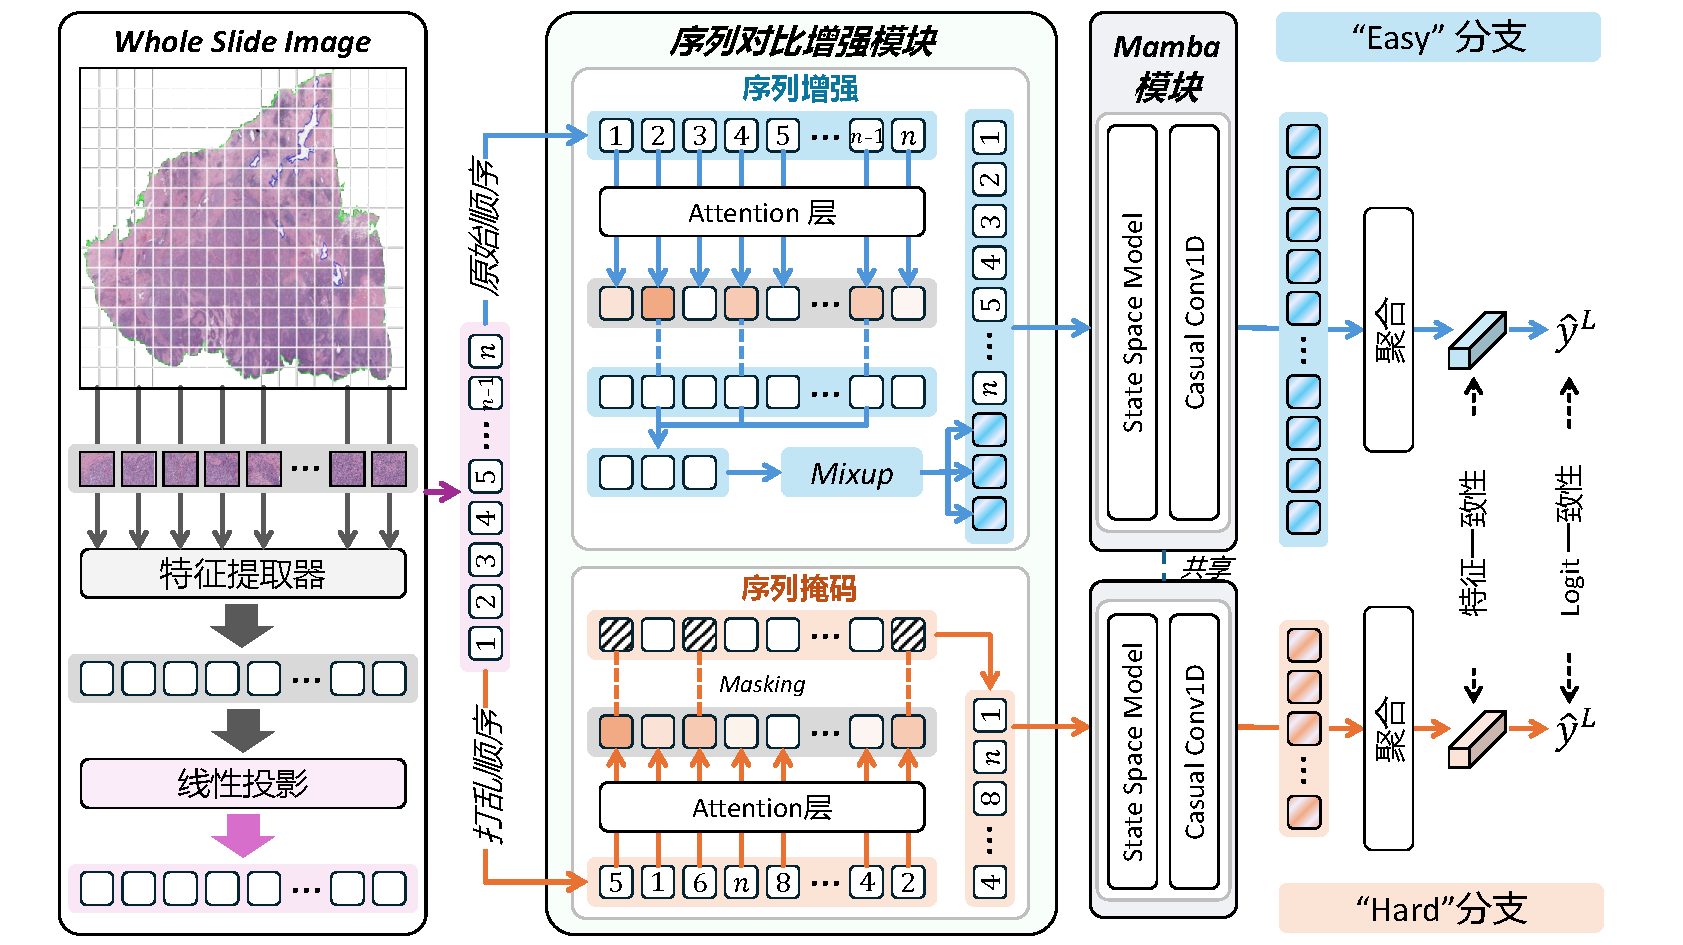
\includegraphics[width=1.0\columnwidth]{figures/SMCMIL.pdf}
  \bicaption[SMC-MIL模型总览图]{SMC-MIL模型总览图。}[Overview of proposed SMC-MIL]{Overview of proposed SMC-MIL.}
  \label{figure3: SMCMIL}
\end{figure}

\subsection[\hspace{-2pt}预处理与特征提取]{{\heiti\zihao{4} \hspace{-8pt}预处理与特征提取}}\label{section4: 预处理与特征提取}

遵从文献~\cite{lu2021data}的设置,每张病理图像被裁剪成一系列$256\times256$的非重叠补丁,放大倍数为$20$倍,同时丢弃背景区域(饱和度$< 15$)。
本章采用ResNet-50~\cite{ROYERCARFAGNI2001253}或UNI~\cite{chen2024towards}作为底层特征提取器$\mathcal{F}(\cdot)$。
因此,本章定义原始扫描序列为:
\begin{equation}
  \mathnormal{Z}=\{z_i\}^{\mathnormal{N}}_{i=1},
\end{equation}
其中$z_i$是$X$的第$i$个实例的提取特征,$N$是实例的个数。
另一个扫描序列定义为$Z'=Resort(Z)$(即$Z'$通过对第一个扫描序列的顺序进行随机重排获得,$Resort(\cdot)$表示随机重排操作)。

\subsection[\hspace{-2pt}基于Mamba的双分支对比架构]{{\heiti\zihao{4} \hspace{-8pt}基于Mamba的双分支对比架构}}\label{section4: 基于Mamba的双分支对比架构}

通过进行序列对比学习,引导Mamba学习扫描不变的包特征。
在该方法中,本章设计了一个双分支实例序列对比学习框架,旨在实现两个极端不同的输入实例序列之间的一致性,并消除序列排列对最终包决策的影响。

假设差异化序列对比增强模块为$S(\cdot)$,则通过差异化序列生成模块可得到两个极端不同的序列:
\begin{equation}
  \begin{aligned} 
    Z_1&=S(Z),\\
    Z_2&=S(Z').
\end{aligned}
\end{equation}
给定一个Mamba模块$\mathrm{\Psi}\left(\cdot\right)$与一个注意力聚合模块$\phi\left(\cdot\right)$,分别对实例序列进行实例关键建模和特征聚合,
为了方便后续表示,该聚合过程记作$\rho\left(\cdot\right)$,统称为Mamba聚合器。
根据上述步骤,则差异化的两个序列分支的包特征分别为:
\begin{equation}
  \begin{aligned} 
  \mathbf{b_1}=\rho(Z_1),\\
  \mathbf{b_2}=\rho(Z_2).
\end{aligned}
\end{equation}

这两个特征都是同一个病理图像的有效表示,因此应该反映一致的视觉内容,本章称之为特征一致性。

给定一个分类器$\mathcal{C}(\cdot)$,分别对这些特征进行分类,获取其分类标签:
\begin{equation}
  \begin{aligned} 
    {\hat{Y}}_1=\mathcal{C}(\mathbf{b_1}),\\
    {\hat{Y}}_l=\mathcal{C}(\mathbf{b_2}).
\end{aligned}
\end{equation}
同样的,这两个标签应该反映一致分类结果,本章称之为标签一致性。

通过特征一致性和标签一致性的约束,反向优化引导Mamba架构学习到与扫描无关的包特征,从根本上突破Mamba架构对输入顺序的依赖,使Mamba架构更适配高分辨率病理图像分类任务。

\subsection[\hspace{-2pt}差异化序列生成(简单与困难分支)]{{\heiti\zihao{4} \hspace{-8pt}差异化序列生成(简单与困难分支)}}\label{section4: 差异化序列生成(简单与困难分支)}

基于扫描序列的顺序、长度以及发现判别区域的难易程度的三个角度,本章提出了一种序列对比度增强方法进行差异化序列生成,即构造“Easy”分支和“Hard”分支。
根据所在分支的不同,上小节提到的序列对比增强模块$S(\cdot)$,可分为两个子模块:序列增强模块$S_A(\cdot)$和序列掩码模块$S_M(\cdot)$。
下面分别详细介绍这两个部分。

\textbf{序列增强 (“Easy” 分支)} 

如图\ref{figure3: SMCMIL}顶部所示,本章设计了一个基于注意力的序列增强模块来构建“Easy”分支。其核心思想是使用注意力机制识别高关注实例,然后通过Mixup对这些已识别的实例执行实例级增强。
此过程生成新实例来补充原始序列。本章将每个实例的注意力得分定义为:
\begin{equation}
  \mathnormal{A}=[a_1,...,a_i,...,a_N]=\mathnormal{\phi}(\mathnormal{Z}),
  \label{eq8}
  \end{equation}
其中$\mathnormal{\phi}(\cdot)$为注意力模块。然后将其进行排序:
\begin{equation}
  \mathnormal{I}=[i_1,i_2,...,i_N]=Sort(\mathnormal{A}),
  \label{eq9}
  \end{equation}
其中$i_1$为注意力得分最高实例的索引,$i_N$为得分最低实例的索引。
本章将实例的$\alpha\%$作为进行序列增强的实例。
其对应的索引是$\lfloor \alpha\% \times N \rfloor$,其对应的实例注意力分数是$I_h=[i_t]^{\lfloor \alpha\% \times N \rfloor}_{t=1}$。则增强序列可表示为:
\begin{equation}
  \mathnormal{Z_{easy}}\leftarrow S_A(Z):=concat\{\varphi(Z_{\mathnormal{I}_h}),Z\},
  \label{eq10}
  \end{equation}
其中$\varphi(\cdot)$是所选实例上的Mixup操作,$S_A(\cdot)$是序列增强模块,$concat$则代表将进行Mixup后的实例同样拼接到原本实例序列上。
注意,这里的注意力机制与后续聚合模块中的注意力模型共享参数。
因此,在“Easy”分支中输入Mamba的序列长度为$\lfloor \alpha\% \times N \rfloor + N$。

\textbf{序列掩码(“Hard”分支)} 

如图\ref{figure3: SMCMIL}底部所示,本章采用基于注意力的掩蔽机制来掩盖“Hard”分支中容易区分的实例,迫使Mamba增强其鉴别可判别性区域的能力。对于分类模型,本章认为具有最高和最低关注值的实例是最容易区分的。
因此,本章试图掩盖这些实例,以迫使模型学习更精确的分类边界。具体来说,本章生成一个$n$维掩码向量$M$如下所示:
  \begin{equation}
    \mathnormal{M}=[m_1,...,m_i,...,m_N],
    \label{eq11}
    \end{equation}
其中$m_i \in \{0,1\}$。如果$m_i$ = 1,则第$i$个实例被保留;$m_i$ = 0时,第$i$个实例被掩码。
本章将高关注值和低关注值的掩码率分别设置为$\beta_h\%$ 和 $\beta_l\%$。
那么,高值对应的序列下标为$I_{\beta_h}=[i_t]^{\lfloor \beta_h\%\times N \rfloor}_{t=1}$,低值对应的序列下标为 $I_{\beta_l}=[i_t]^{N}_{t=N-\lfloor \beta_l\%\times N \rfloor}$。因此,
\begin{equation}
  \mathnormal{m_i}=\left \{
  \begin{array}{cl}
      0 &  i\in I_{\beta_h} \cup  I_{\beta_l}, \\
      1 & other.
  \end{array}\right.
  \label{eq12}
  \end{equation}
最后,掩码后的序列可以表示为:
\begin{equation}
  \mathnormal{Z_{hard}}\leftarrow S_M(Z'):=M\cdot \mathnormal{Z'},
  \label{eq13}
  \end{equation}
其中$S_M(\cdot)$是序列掩码模块。为了便于讨论,本文假设$\beta_h=\beta_l$。

“Easy”分支保留了原本的序列顺序,同时增加了序列长度,并且通过Mixup操作添加了多样性,降低了Mamba捕获可判别性区域的难度;
“Hard”分支打乱了原本的序列顺序,同时缩减了序列长度,并且通过掩盖掉易于分辨的实例,提高了Mamba捕获可判别性区域的难度。
上下两个分支形成了鲜明的对比。如此差异化的序列分支,加大了对比学习任务的难度,迫使Mamba学习到更清晰的分类边界,以提高模型鲁棒性。

\subsection[\hspace{-2pt}基于Mamba的实例聚合]{{\heiti\zihao{4} \hspace{-8pt}基于Mamba的实例聚合}}\label{section4: 基于Mamba的实例聚合}
本小节介绍基于Mamba的实例聚合,即上文所提到的Mamba聚合器$\rho\left(\cdot\right)$。
如上所述,“Easy”和“Hard”分支的输入实例序列分别为$\mathnormal{Z_{easy}}$和$\mathnormal{Z_{hard}}$。$\Psi(\cdot)$是上文提到的一个Mamba块。这两个分支的包表示可以通过执行基于注意力机制的聚合来获得,
\begin{equation}
  \begin{aligned}
      &\mathbf{b}_1=\mathnormal{A_1} \cdot \Psi(\mathnormal{Z_{easy}})=\phi(\Psi(S_A(Z)))\cdot \Psi(S_A(Z)), \\
      &\mathbf{b}_2=\mathnormal{A_2} \cdot \Psi(\mathnormal{Z_{hard}})=\phi(\Psi(S_M(Z')))\cdot \Psi(S_M(Z')),
  \end{aligned}
  \label{eq6}
\end{equation}
其中$\mathnormal{A_1}$和$\mathnormal{A_2}$分别是$ \Psi(\mathnormal{Z_{easy}})$和$ \Psi(\mathnormal{Z_{easy}})$的注意力分数。类似地,它们的预测包标签可以通过将包的表示输入分类器$\mathcal{C}(\cdot)$得到,
\begin{equation}
  \begin{aligned}
      &\hat{Y}_1\leftarrow \mathcal{C}(\mathbf{b}_1):=\mathcal{C}(\mathnormal{A_1}\cdot \Psi(\mathnormal{Z_{easy}})),\\
      &\hat{Y}_2\leftarrow \mathcal{C}(\mathbf{b}_2):=\mathcal{C}(\mathnormal{A_2} \cdot \Psi(\mathnormal{Z_{hard}})).
  \end{aligned}
  \label{eq7}
  \end{equation} 

\subsection[\hspace{-2pt}基于一致性的模型优化]{{\heiti\zihao{4} \hspace{-8pt}基于一致性的模型优化}}\label{section4: 基于一致性的模型优化}

由于这两个分支的扫描序列都来自同一个包,因此它们的包表示和分类应该是一致的。它们的包表示的一致性损失为:
\begin{equation}
    \mathcal{L}_{b_{con}}=-%\frac{softmax(\mathbf{b}_1)log(\mathbf{b}_2)+softmax(\mathbf{b}_2)log(\mathbf{b}_1)}{2} , 
    %\frac{1}{2}[\mathrm{Softmax}(\mathbf{b}_1)\log(\mathbf{b}_2)+\mathrm{Softmax}(\mathbf{b}_2)\log(\mathbf{b}_1) ]
    \frac{\mathrm{Softmax}(\mathbf{b}_1)\log(\mathbf{b}_2)+\mathrm{Softmax}(\mathbf{b}_2)\log(\mathbf{b}_1)}{2}.
    \label{eq15}
  \end{equation}
而它们的包分类的一致性损失为:
\begin{equation}
    %\mathcal{L}_{l_{con}}=-(\mathrm{softmax}(\hat{Y}_1)\mathrm{log}(\hat{Y}_2)+\mathrm{softmax}(\hat{Y}_2)\mathrm{log}(\hat{Y}_1))/2.
    %\mathcal{L}_{l_{con}}=-\frac{1}{2}[\mathrm{Softmax}(\hat{Y}_1)\log(\hat{Y}_2)+\mathrm{Softmax}(\hat{Y}_2)\log(\hat{Y}_1)].
    \mathcal{L}_{l_{con}}=-\frac{\mathrm{Softmax}(\hat{Y}_1)\log(\hat{Y}_2)+\mathrm{Softmax}(\hat{Y}_2)\log(\hat{Y}_1)}{2}.
    \label{eq16}
  \end{equation}
除了一致性损失之外,本章还向“Easy”分支引入了分类损失,以确保预测标签与其真实值之间的一致性,
\begin{equation}
	\mathcal{L}_{cls}=Y \log\hat{Y}_1+(1-Y)\log(1-\hat{Y}_1),
	\label{eq14}
\end{equation}
其中$Y$是真实值。
综上所述,该模型可通过处理以下优化问题得到:
\begin{equation}
	\{\hat{\Psi},\hat{\phi},\hat{\mathcal{C}}\}\leftarrow \arg\mathop{\min}\limits_{\hat{\Psi},\hat{\phi},\hat{\mathcal{C}}} \mathcal{L}=\mathcal{L}_{cls}+\gamma (\mathcal{L}_{b_{con}}+\mathcal{L}_{l_{con}}),
	\label{eq17}
\end{equation}
其中$\hat{\Psi},\hat{\phi},\hat{\mathcal{C}}$是本章网络的参数,$\gamma$是平衡分类损失和一致性损失的参数。

\subsection[\hspace{-2pt}模型推理]{{\heiti\zihao{4} \hspace{-8pt}模型推理}}\label{section4: 模型推理}

在模型训练阶段,本章采用双分支对比学习架构,通过约束其中特征一致性和标签一致性,反向梯度优化Mamba架构。
而在模型推理环节,本章仅借助单分支 Mamba 模型来执行图像的标签预测工作。详细来讲,本章分别对以下两种推理模式进行了尝试:


\begin{figure}[h]
  \centering
  \captionsetup{font={small, stretch=1.312}}
  \subfloat[采用序列增强模块进行推理]{
		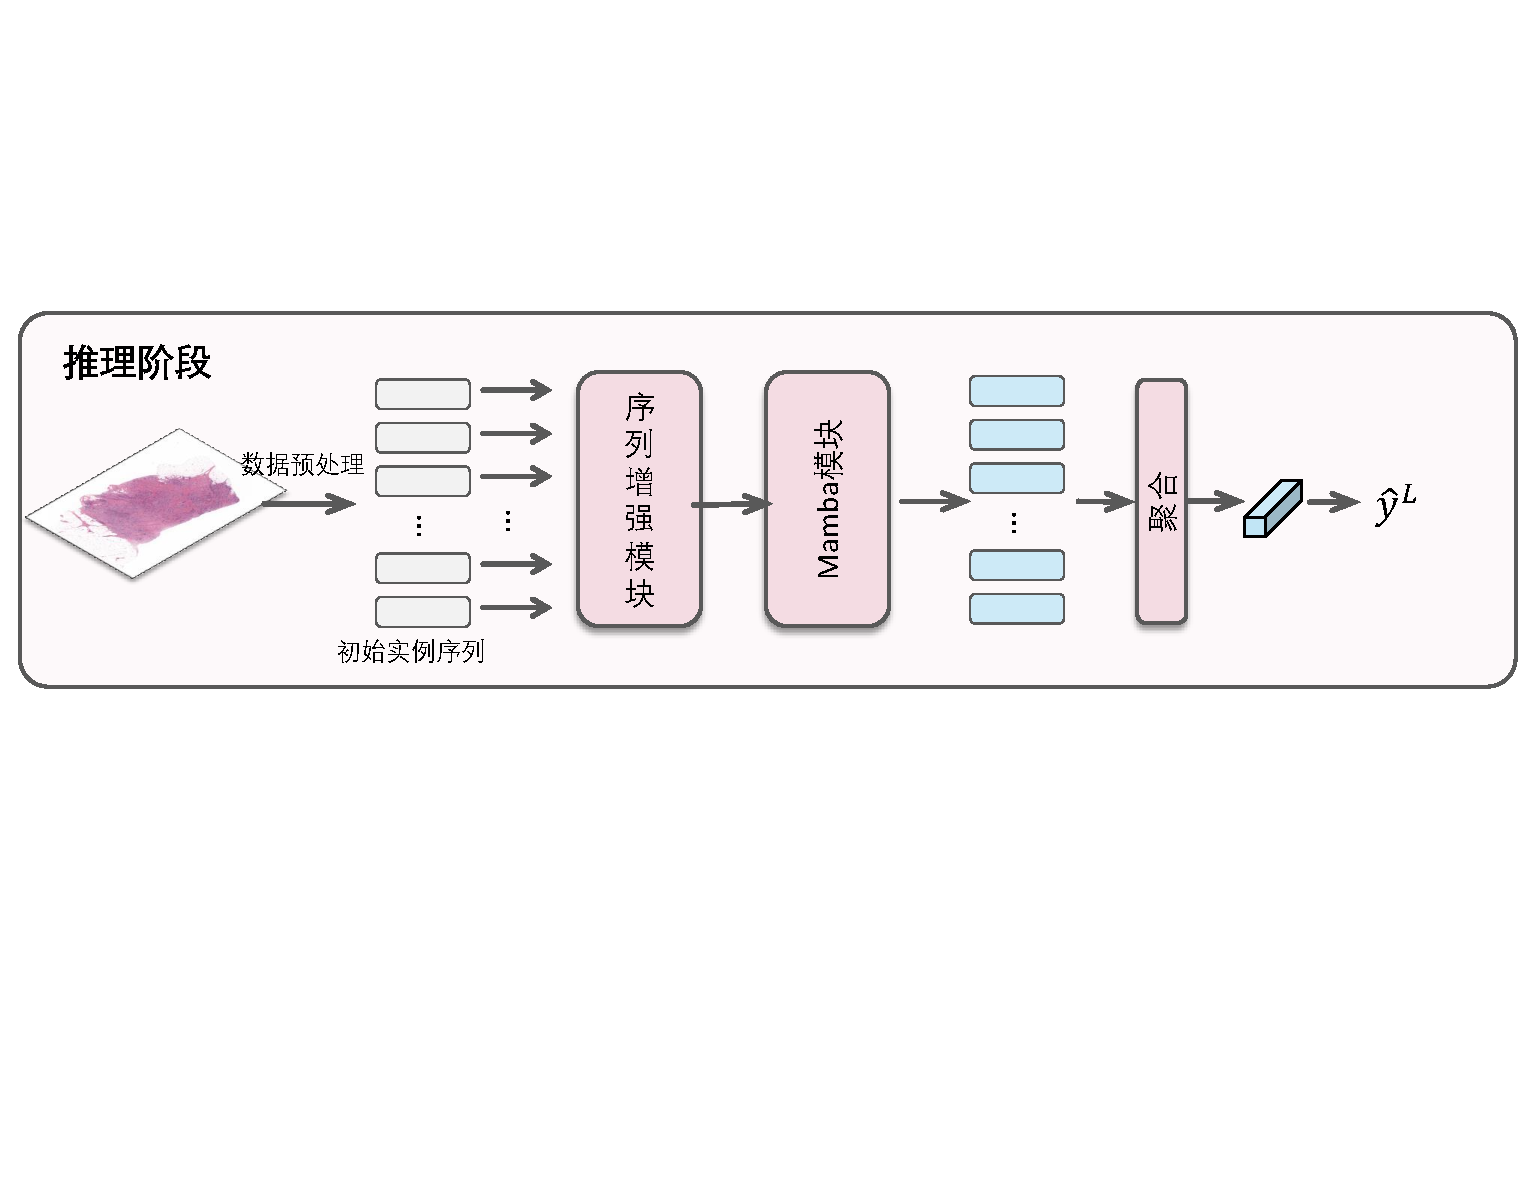
\includegraphics[width=1.0\columnwidth]{figures/基于easy分支的推理阶段.pdf}
    \label{figure3:推理流程1}
    }\\
  \subfloat[不采用序列增强模块进行推理]{
		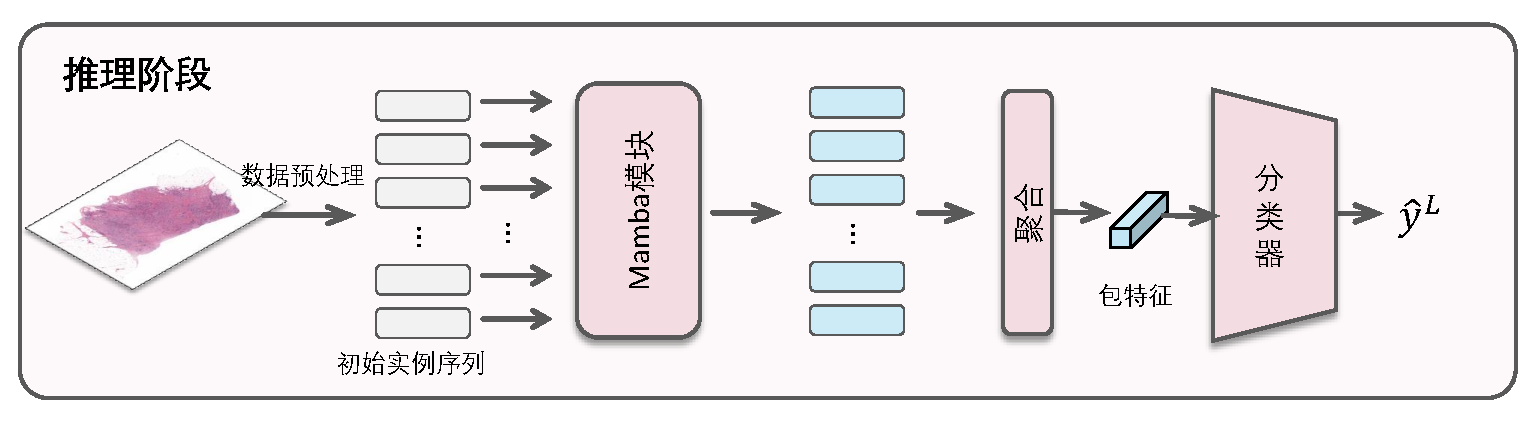
\includegraphics[width=1.0\columnwidth]{figures/基于Mamba的推理阶段.pdf}
    \label{figure3:推理流程2}
    }
  %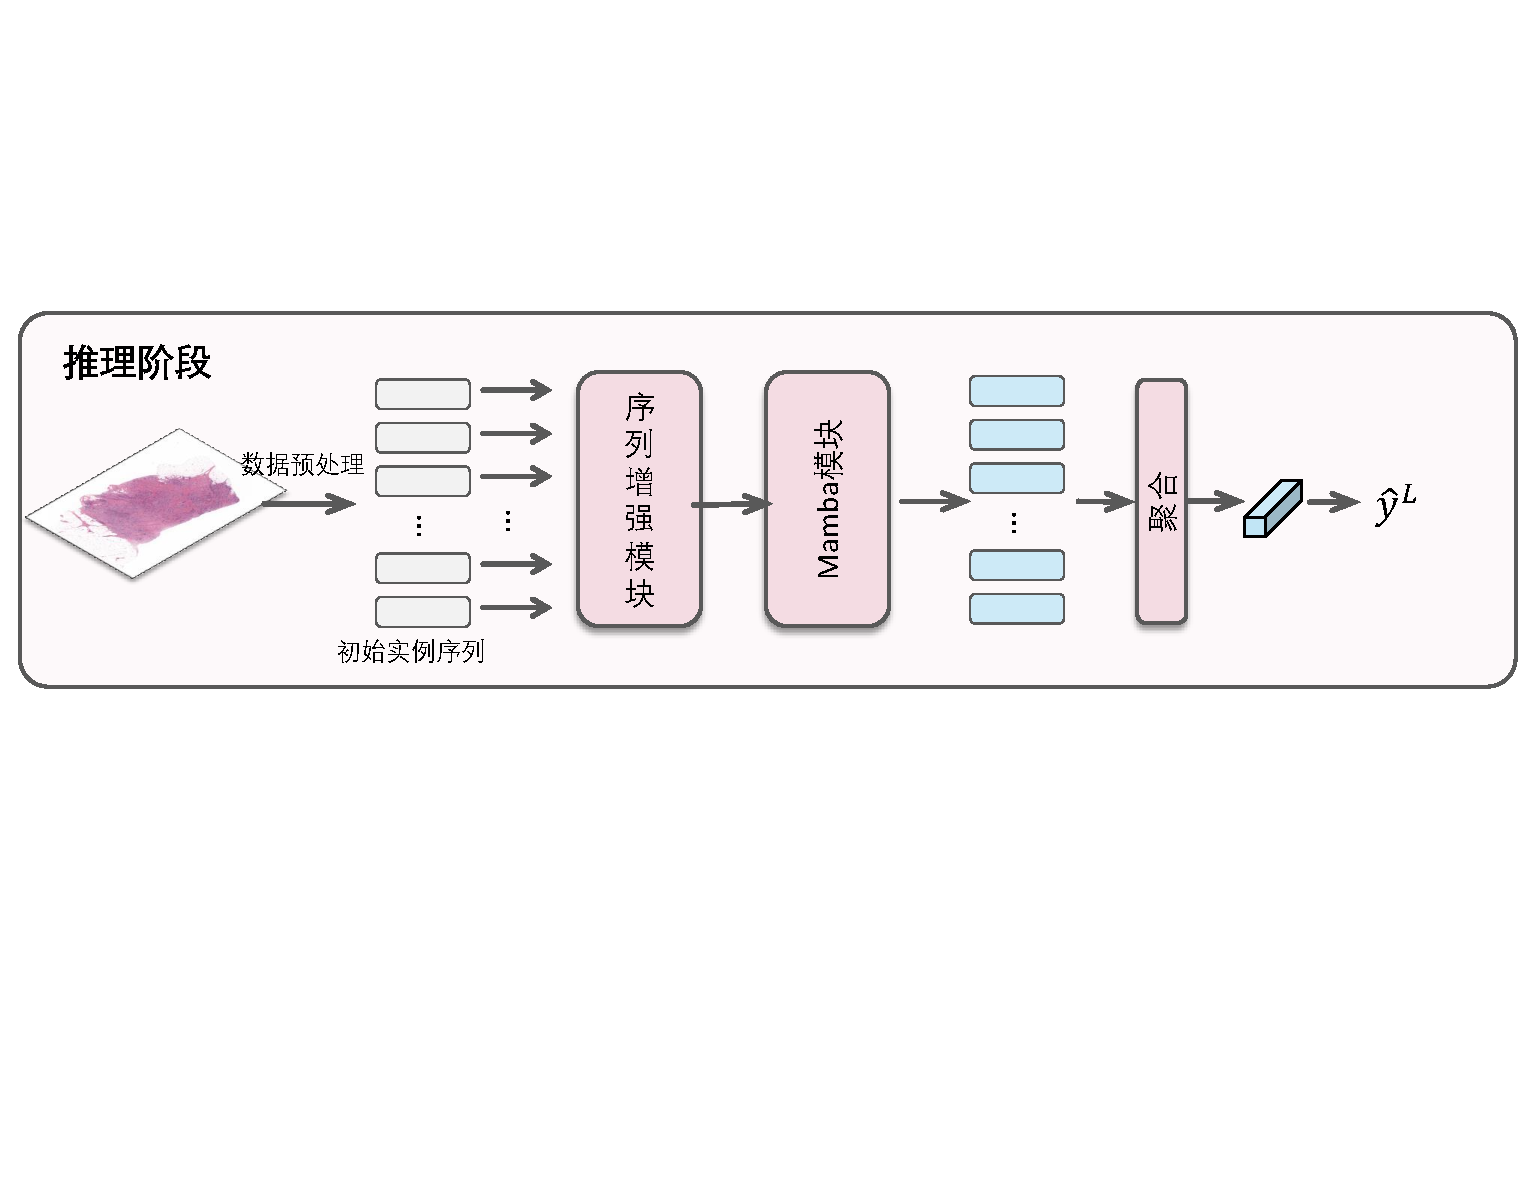
\includegraphics[width=1.0\columnwidth]{figures/基于easy分支的推理阶段.pdf}
  \bicaption[SMC-MIL模型推理流程示意图]{SMC-MIL模型推理流程示意图。}[Schematic diagram of SMC-MIL model inference process]{Schematic diagram of SMC-MIL model inference process.}
  \label{figure3: 推理流程}
\end{figure}

\textbf{采用序列增强模块进行推理:} 给定一张图像$X$经过图像预处理操作后得到实例特征序列,送入到序列增强模块获得新的序列。
继续送入Mamba模块后建模各实例间信息,建模出更好的特征。
最终,通过聚合模块输出包特征,将其输入分类网络以生成最终预测结果。
具体推理流程详见图\ref{figure3:推理流程1}。

\textbf{不采用序列增强模块进行推理:} 本章还尝试了不采用序列增强模块直接进行输入至Mamba模块进行推理。推理流程详情见图\ref{figure3:推理流程2}所示。

在不特别说明的情况下,本文采用序列增强模块进行推理。

\section[\hspace{-2pt}实验设置及结果分析]{{\heiti\zihao{-3} \hspace{-8pt}实验设置及结果分析}}\label{section4: 实验设置及结果分析}

在本节中,首先介绍了本章方法的实验设置,包括实验使用数据集、评估指标和实验细节,
然后分析了基于扫描不变性Mamba的高分辨率病理图像分类实验结果,接下来对模型的各个模块以及超参数进行了消融实验和分析,最后对模型所关注的重点区域进行了可视化分析。

\subsection[\hspace{-2pt}实验设置]{{\heiti\zihao{4} \hspace{-8pt}实验设置}}\label{section4: 实验设置}
\textbf{(1)实验环境}


本章实验依托于和上一章实验同样的设置环境和平台。%该平台搭载AMD Ryzen 5700X 20 核中央处理器与 3 块 NVIDIA RTX 3090 图形处理器。
%实验框架基于 Python 编程语言构建,采用 OpenSlide 库实现病理图像的高效读取,基于 Matplotlib 库完成数据可视化。
详细的实验环境参数配置见表\ref{table4: env}:

\begin{table}[h!]
  \small    % 设置表格字体为5号
  \setstretch{1.245}        % 设置具有指定弹力的橡皮长度(原行宽的1.2倍)
  \captionsetup{font={small, stretch=1.512}}
  \centering
  \bicaption[基于扫描不变性Mamba的高分辨率病理图像分类研究的实验环境及配置 ]{基于扫描不变性Mamba的高分辨率病理图像分类的实验环境及配置}[Experimental environment and configuration of SMC-MIL ]{Experimental environment and configuration of SMC-MIL}
  \begin{tabularx}{\textwidth}{CcCC}
  \toprule
  设备     & 配置               & 版本          & 数量 \\ 
  \midrule
  操作系统   & Ubuntu           & 20.04.4 LTS & 1  \\
  CPU    & AMD Ryzen 5700X  & -           & 1  \\
  GPU    & GeForce RTX 3090 & -           & 3  \\
  IDE    & VsCode           & 1.86.2      & 1  \\
  编程语言   & Python           & 3.10.11       & -  \\
  深度学习框架 & Pytorch          & 2.0.1       & -  \\
  \bottomrule
  \end{tabularx}
  \label{table4: env}
  \end{table}


\textbf{(2)数据集}

本章同样通过三个WSI分析子任务来评估SMC-MIL模型:癌症诊断、亚型分类和生存预测。
对于癌症诊断任务,本章采用和上一章同样的设置,采用CAMELYON数据集进行评估。
对于分型任务,本章使用 TCGA-NSCLC、TCGA-BRCA和BRACS~\cite{brancati2022bracs}数据集。
同时为了评估生存预测的准确性,本章使用 TCGA-LUAD,TCGA-LUSC,TCGA-BLCA来评估生存预测任务的性能。

\textbf{(3)评估指标}

对于诊断和分型,本章利用Accuracy、AUC和F1-score来评估模型的性能,其中AUC是本章主要的评价指标,在消融实验的讨论中,本章仅报告AUC。对于生存预测,本章报告了所有数据集的C-index。默认情况下,本章采用5折交叉验证,这与性能比较的基线方法一致。
具体来说,对于BRACS数据集,本章也遵循了来自官方的划分方案,在官方分区中将数据集分为395:65:87的训练集、验证集和测试集。
本章进行了三次独立的重复实验,以尽量减少官方划分的随机影响。此外,为了在实验中保持与其他数据集的一致性,本章还对BRACS的7类分类任务进行了5次交叉验证实验,标记为BRACS-7$^\star$,并报告在表\ref{table4: BRACS_7}中。

%\textbf{(4)实施细节}

%按照之前的工作\cite{lu2021data,zhang2022dtfd,tang2023multiple},每个WSI病理图像被裁剪成一系列$256 \times 256$的不重叠的贴片,放大倍数为20倍,同时丢弃背景区域(饱和度$< 15$)。
%本章使用在ImageNet \cite{deng2009imagenet}中预训练的ResNet-50模型\cite{he2016deep}和在$1\times 10^6$ WSIs的$1\times 10^8$ Patches的大型内部组织学数据集上预训练的最新基础模型UNI \cite{chen2024towards}作为骨干网络,
%从每个Patch中提取初始特征向量,其维度为1024。
%初始特征向量随后通过全连接层降为512维表示。
%在处理所有数据集时,将学习率设定为$2 \times 10^{\textnormal{-}4}$,权重衰减系数设为$10^{\textnormal{-}5}$。学习率的调整采用余弦退火策略,该策略能够使学习率随着训练轮次的增加而动态、平滑地变化,有助于模型更有效地收敛。
%所有模型均运用早停策略开展了 200 个轮次的训练。早停策略可在验证集性能不再提升时及时停止训练,防止模型过拟合,从而保证模型在测试集上具备良好的泛化能力。
%本章未引入梯度裁剪或梯度累积等优化技巧,以确保实验结果的纯粹性与方法对比的公平性。所有模型均基于标准训练流程完成参数优化,未采用任何额外的正则化技术或训练技巧。批量大小设置为1。
%所有实验均使用RTX 3090 GPU,在Ubuntu 20.04.4、Python版本3.10.11和PyTorch版本2.0.1的环境下进行。

\textbf{(4)实施细节与对比方法}

在实施细节上,本章采用与上一章实验同样的实验细节设置。
在对比方法上,本文采用了10种广泛使用的MIL方法以及上一章研究的方法与本章方法进行比较。
其中包括: AB-MIL~\cite{ilse2018attention},  CLAM~\cite{lu2021data}, 
DSMIL~\cite{li2021dual}, TransMIL~\cite{shao2021transmil}, DTFD-MIL ~\cite{zhang2022dtfd},
IBMIL ~\cite{lin2023interventional}, MHIM-MIL ~\cite{tang2023multiple},
SRMamba~\cite{yang2024mambamil}, WIKG~\cite{li2024dynamic},
R$^2$T-MIL~\cite{tang2024feature}和M$^2$S-MIL。
其中SRMamba与上一章所提出的方法M$^2$S-MIL是基于Mamba架构的方法,也是本章主要的基准方法。
本文在相同的设置下复现了这些方法的结果以进行比较。
\subsection[\hspace{-2pt}基准数据集实验结果]{{\heiti\zihao{4} \hspace{-8pt}基准数据集实验结果}}\label{section4: 基准数据集实验结果}

\textbf{(1)癌症诊断和分型}


{
\large    % 设置表格字体为5号
\setstretch{1.245}        % 设置具有指定弹力的橡皮长度(原行宽的1.2倍)
%\setlength{\tabcolsep}{10pt}
\captionsetup{font={small, stretch=1.512}}
\begin{xltabular}{\textwidth}{XCCC}
  \bilingualcaption{SMC-MIL在CAMELYON数据集的癌症诊断性能比较(\%)}{SMC-MIL在CAMELYON数据集的癌症诊断性能比较(\%)。最优结果用粗体表示,次优结果使用下划线表示。}{Comparison of cancer diagnostic performance of SMC-MIL on the CAMELYON dataset (\%). The optimal experimental results are marked in bold, and the sub-optimal are underlined.}
  \label{table4: CAMELYON} \\
  \toprule
  方法   & Accuracy          & AUC      & F1-score  \\ 
  \midrule
  \endfirsthead

  \multicolumn{4}{c}{\tablename \thetable{} (续)} \\ % 第一行标题
  \multicolumn{4}{c}{Table \thetable{} (continued)} \\ % 第二行标题

  \toprule
  方法   & Accuracy          & AUC      & F1-score  \\ 
  \midrule
  \endhead

  % \midrule \multicolumn{3}{r}{{接下页}} \\ 
  \bottomrule
  \endfoot

  \bottomrule
  \endlastfoot

  % 添加你的内容
  AB-MIL~\cite{ilse2018attention}& 88.08$\pm$1.87& 91.18$\pm$1.60&83.59$\pm$2.75\\
  CLAM~\cite{lu2021data}&                87.98$\pm$2.17& 91.70$\pm$2.15&  83.38$\pm$3.09\\
  
  DSMIL~\cite{li2021dual}          & 88.42$\pm$1.77& 91.50$\pm$1.23& 83.82$\pm$2.95\\
  TransMIL~\cite{shao2021transmil} & 88.75$\pm$1.04& 91.82$\pm$1.82& 84.47$\pm$1.57\\
  DTFD-MIL~\cite{zhang2022dtfd}    & 88.07$\pm$1.13&91.61$\pm$1.73& 83.24$\pm$1.67\\
  MHIM-MIL~\cite{tang2023multiple}    & 89.42$\pm$1.16& 92.55$\pm$1.11& 84.63$\pm$2.13\\
  IBMIL~\cite{lin2023interventional}    & 88.98$\pm$2.08&91.75$\pm$2.09& 84.61$\pm$3.07\\
  SRMamba~\cite{yang2024mambamil}& 88.75$\pm$1.47 &91.82$\pm$0.93 & 84.27$\pm$2.08\\
  WiKG ~\cite{li2024dynamic} & 88.19$\pm$2.30& 91.42$\pm$1.44& 82.93$\pm$3.41 \\
  R$^2$T-MIL ~\cite{tang2024feature} & 89.20$\pm$1.48 & 92.29$\pm$1.32 & 85.20$\pm$1.86\\
  %\textbf{M$^2$S-MIL}
  第三章方法 & \underline{89.76$\pm$1.33}& \underline{93.02$\pm$1.20}& \underline{85.48$\pm$2.43}\\
  \textbf{SMC-MIL(Ours)}& \textbf{89.97$\pm$1.78}& \textbf{93.81$\pm$1.65}& \textbf{85.76$\pm$1.77}\\

\end{xltabular}}

{
  \large
%\small    % 设置表格字体为5号
\setstretch{1.245}        % 设置具有指定弹力的橡皮长度(原行宽的1.2倍)
\captionsetup{font={small, stretch=1.512}}
\begin{xltabular}{\textwidth}{XCCC}
  \bilingualcaption{SMC-MIL在TCGA-NSCLC数据集的亚型分类性能比较(\%)}{SMC-MIL在TCGA-NSCLC数据集的亚型分类性能比较(\%)。最优结果用粗体表示,次优结果使用下划线表示。}{Comparison of sub-typing performance of SMC-MIL on the TCGA-NSCLC dataset (\%). The optimal experimental results are marked in bold, and the sub-optimal are underlined.}
  \label{table4: NSCLC} \\
  \toprule
  方法   & Accuracy          & AUC      & F1-score  \\ 
  \midrule
  \endfirsthead

  \multicolumn{4}{c}{\tablename \thetable{} (续)} \\ % 第一行标题
  \multicolumn{4}{c}{Table \thetable{} (continued)} \\ % 第二行标题

  \toprule
  方法   &Accuracy          & AUC      & F1-score  \\ 
  \midrule
  \endhead

  % \midrule \multicolumn{3}{r}{{接下页}} \\ 
  \bottomrule
  \endfoot

  \bottomrule
  \endlastfoot

  % 添加你的内容
  AB-MIL~\cite{ilse2018attention}& 90.42$\pm$1.76&95.23$\pm$1.46&89.93$\pm$1.80\\
  CLAM~\cite{lu2021data}& 87.98$\pm$2.17& 91.70$\pm$2.15&  83.38$\pm$3.09\\
  
  DSMIL~\cite{li2021dual}          & 90.33$\pm$1.97&95.68$\pm$1.01&89.91$\pm$2.19\\
  TransMIL~\cite{shao2021transmil} &  90.13$\pm$1.07&94.92$\pm$1.02&89.52$\pm$1.07\\
  DTFD-MIL~\cite{zhang2022dtfd}    &90.71$\pm$1.66&95.64$\pm$1.44&90.29$\pm$1.83\\
  MHIM-MIL~\cite{tang2023multiple}    & 91.18$\pm$1.79&95.84$\pm$1.41&90.91$\pm$1.97\\
  IBMIL~\cite{lin2023interventional}    &89.76$\pm $2.29&95.49$\pm$1.18&89.43$\pm$2.21\\
  SRMamba~\cite{yang2024mambamil}&  90.43$\pm$3.26&95.07$\pm$1.96&90.18$\pm$3.21\\
  WiKG ~\cite{li2024dynamic}&  89.67$\pm$2.49&94.96$\pm$1.66&89.53$\pm$2.43\\
  R$^2$T-MIL ~\cite{tang2024feature}& 90.81$\pm$2.41& {96.20$\pm$1.16}&90.49$\pm$2.41\\

  %\textbf{M$^2$S-MIL}
  第三章方法 &  \underline{91.48$\pm$2.29}& \underline{96.65$\pm$1.08}&\underline{91.19$\pm$2.29}\\
   \textbf{SMC-MIL(Ours)}&  \textbf{91.85$\pm$2.37}& \textbf{97.10$\pm$1.46}&\textbf{91.61$\pm$2.40}\\

\end{xltabular}}

{
  \large
%\small    % 设置表格字体为5号
\setstretch{1.245}        % 设置具有指定弹力的橡皮长度(原行宽的1.2倍)
\captionsetup{font={small, stretch=1.512}}
\begin{xltabular}{\textwidth}{XCCC}
  \bilingualcaption{SMC-MIL在TCGA-BRCA数据集的亚型分类性能比较(\%)}{SMC-MIL在TCGA-BRCA数据集的亚型分类性能比较(\%)。最优结果用粗体表示,次优结果使用下划线表示。}{Comparison of  sub-typing performance of SMC-MIL on the TCGA-BRCA dataset (\%). The optimal experimental results are marked in bold, and the sub-optimal are underlined.}
  \label{table4: BRCA} \\
  \toprule
  方法   & Accuracy          & AUC      & F1-score  \\ 
  \midrule
  \endfirsthead

  \multicolumn{4}{c}{\tablename \thetable{} (续)} \\ % 第一行标题
  \multicolumn{4}{c}{Table \thetable{} (continued)} \\ % 第二行标题

  \toprule
  方法   &Accuracy          & AUC      & F1-score  \\ 
  \midrule
  \endhead

  % \midrule \multicolumn{3}{r}{{接下页}} \\ 
  \bottomrule
  \endfoot

  \bottomrule
  \endlastfoot

  % 添加你的内容
  AB-MIL~\cite{ilse2018attention}& 86.80$\pm$2.56&91.17$\pm$1.69&72.42$\pm$3.48\\
  CLAM~\cite{lu2021data}&      86.15$\pm$3.98&91.38$\pm$1.67&72.29$\pm$4.21\\
  
  DSMIL~\cite{li2021dual}          &  86.58$\pm$3.86&91.80$\pm$2.09&72.63$\pm$4.49\\
  TransMIL~\cite{shao2021transmil} & 86.22$\pm$3.30&91.61$\pm$1.81&72.20$\pm$4.28\\
  DTFD-MIL~\cite{zhang2022dtfd}    &  86.04$\pm$3.05&91.34$\pm$1.95&70.76$\pm$4.20\\
  MHIM-MIL~\cite{tang2023multiple} &  86.80$\pm$2.56&92.24$\pm$1.63&74.77$\pm$7.72\\
  IBMIL~\cite{lin2023interventional} &  85.54$\pm$3.20 &91.41$\pm$2.20 &71.14$\pm$3.60 \\
  SRMamba ~\cite{yang2024mambamil}& 88.14$\pm$3.05&93.31$\pm$1.40&75.61$\pm$4.00\\
  WiKG ~\cite{li2024dynamic}& 88.53$\pm$2.28 &92.14$\pm$2.06&75.11$\pm$3.98\\
  R$^2$T-MIL ~\cite{tang2024feature}& 88.25$\pm$2.06 & 92.58$\pm$1.75 & 75.15$\pm$2.91\\

  %\textbf{M$^2$S-MIL}
  第三章方法 &  \underline{89.26$\pm$2.37}& \underline{93.50$\pm$1.70}& \underline{76.62$\pm$3.47}\\
  \textbf{SMC-MIL(our)}&  \textbf{90.16$\pm$1.83}& \textbf{93.98$\pm$1.02}& \textbf{78.11$\pm$3.30}\\
  

\end{xltabular}}


{
\large    % 设置表格字体为5号
\setstretch{1.245}        % 设置具有指定弹力的橡皮长度(原行宽的1.2倍)
%\setlength{\tabcolsep}{10pt}
\captionsetup{font={small, stretch=1.512}}
\begin{xltabular}{\textwidth}{XCCC}
  \bilingualcaption{SMC-MIL在BRACS数据集官方划分下的粗粒度分类性能对比(\%)}{SMC-MIL在BRACS数据集官方划分下的粗粒度分类(三分类)性能对比(\%)。最优结果用粗体表示,次优结果使用下划线表示。}{Performance comparison of SMC-MIL coarse-grained classification (3-class) under the official classification of BRACS dataset (\%)). The optimal experimental results are marked in bold, and the sub-optimal are underlined.}
  \label{table4: BRACS3} \\
  \toprule
  方法   & Accuracy          & AUC      & F1-score  \\ 
  \midrule
  \endfirsthead

  \multicolumn{4}{c}{\tablename \thetable{} (续)} \\ % 第一行标题
  \multicolumn{4}{c}{Table \thetable{} (continued)} \\ % 第二行标题

  \toprule
  方法   & Accuracy          & AUC      & F1-score  \\ 
  \midrule
  \endhead

  % \midrule \multicolumn{3}{r}{{接下页}} \\ 
  \bottomrule
  \endfoot

  \bottomrule
  \endlastfoot

  % 添加你的内容
  AB-MIL~\cite{ilse2018attention}& 58.05$\pm$1.44 & 80.68$\pm$0.35&55.83$\pm$1.97 \\
  CLAM~\cite{lu2021data}&  57.85$\pm$0.94 & 83.54$\pm$0.69 & 58.41$\pm$1.08 \\
  
  DSMIL~\cite{li2021dual}          & 55.21$\pm$0.85 & 82.54$\pm$0.57 & 51.67$\pm$0.75\\
  TransMIL~\cite{shao2021transmil} & 54.17$\pm$2.55 & 79.32$\pm$0.31 & 50.68$\pm$2.40  \\
  DTFD-MIL~\cite{zhang2022dtfd}    & 58.22$\pm$6.26 &{85.96$\pm$2.13} &{59.70$\pm$2.86} \\
  MHIM-MIL~\cite{tang2023multiple}    &57.78$\pm$1.28 & 81.03$\pm$0.13 &54.74$\pm$1.56 \\
  IBMIL~\cite{lin2023interventional}    & 58.30$\pm$3.58 & 80.07$\pm$2.42 & 58.27$\pm$4.88\\
  SRMamba ~\cite{yang2024mambamil}& {58.38$\pm$5.21}&83.12$\pm$3.90 & 57.87$\pm$6.94 \\
  WiKG ~\cite{li2024dynamic}& 51.74$\pm$2.46 & 76.71$\pm$1.80 & 48.71$\pm$2.31 \\
  R$^2$T-MIL ~\cite{tang2024feature}& 56.02$\pm$2.36 &82.11$\pm$0.54 & 55.58$\pm$3.65  \\

  %\textbf{M$^2$S-MIL} 
  第三章方法 &\underline{59.38$\pm$1.13} &\underline{86.21$\pm$0.46} & \underline{60.13$\pm$1.79}\\
  \textbf{SMC-MIL(Ours)} &\textbf{59.78$\pm$1.18} &\textbf{87.74$\pm$0.36} & \textbf{61.13$\pm$2.08}\\

\end{xltabular}}

{
\large    % 设置表格字体为5号
\setstretch{1.245}        % 设置具有指定弹力的橡皮长度(原行宽的1.2倍)
%\setlength{\tabcolsep}{10pt}
\captionsetup{font={small, stretch=1.512}}
\begin{xltabular}{\textwidth}{XCCC}
  \bilingualcaption{SMC-MIL在BRACS数据集官方划分下的细粒度分类性能对比(\%)}{SMC-MIL在BRACS数据集官方划分下的细粒度分类(七分类)性能对比(\%)。最优结果用粗体表示,次优结果使用下划线表示。}{Performance comparison of SMC-MIL's fine-grained classification (7-class) under the official classification of BRACS dataset(\%). The optimal experimental results are marked in bold, and the sub-optimal are underlined.}
  \label{table4: BRACS7} \\
  \toprule
  方法   & Accuracy          & AUC      & F1-score  \\ 
  \midrule
  \endfirsthead

  \multicolumn{4}{c}{\tablename \thetable{} (续)} \\ % 第一行标题
  \multicolumn{4}{c}{Table \thetable{} (continued)} \\ % 第二行标题

  \toprule
  方法   & Accuracy          & AUC      & F1-score  \\ 
  \midrule
  \endhead

  % \midrule \multicolumn{3}{r}{{接下页}} \\ 
  \bottomrule
  \endfoot

  \bottomrule
  \endlastfoot

  % 添加你的内容
  AB-MIL~\cite{ilse2018attention}& 30.44$\pm$2.67 & 73.92$\pm$0.29 &28.76$\pm$2.12 \\
  CLAM~\cite{lu2021data}&  \underline{37.60$\pm$1.52} & 76.83$\pm$1.29 &35.68$\pm$2.84 \\
  
  DSMIL~\cite{li2021dual}          & 27.68$\pm$5.10 &76.66$\pm$0.83 &27.56$\pm$4.34\\
  TransMIL~\cite{shao2021transmil} & 26.83$\pm$5.48 &70.34$\pm$2.57 &25.28$\pm$3.15 \\
  DTFD-MIL~\cite{zhang2022dtfd}    & 35.02$\pm$2.76 & \underline{79.17$\pm$0.80} &\underline{35.92$\pm$6.29}\\
  MHIM-MIL~\cite{tang2023multiple} & 34.39$\pm$1.55 &  74.20$\pm$0.46& 33.09$\pm$1.08\\
  IBMIL~\cite{lin2023interventional} & 32.74$\pm$2.36 &74.80$\pm$0.29 &30.58$\pm$2.94 \\
  SRMamba ~\cite{yang2024mambamil}& 33.99$\pm$4.27 &74.92$\pm$2.00 &33.94$\pm$3.26 \\
  WiKG ~\cite{li2024dynamic}& 33.13$\pm$2.43 &74.14$\pm$1.23 &32.93$\pm$4.39\\
  R$^2$T-MIL ~\cite{tang2024feature}& 26.64$\pm$1.02 &74.02$\pm$1.40 &26.67$\pm$1.59 \\
  %\textbf{M$^2$S-MIL}
  第三章方法 &{34.16$\pm$2.04} &{77.37$\pm$1.24} & {34.37$\pm$2.73}\\

  \textbf{SMC-MIL(Ours)}& \textbf{38.29$\pm$0.87}& \textbf{79.57$\pm$0.42}&\textbf{37.93$\pm$1.33}\\

\end{xltabular}}


{
\large    % 设置表格字体为5号
\setstretch{1.245}        % 设置具有指定弹力的橡皮长度(原行宽的1.2倍)
%\setlength{\tabcolsep}{10pt}
\captionsetup{font={small, stretch=1.512}}
\begin{xltabular}{\textwidth}{XCCC}
  \bilingualcaption{SMC-MIL在BRACS数据集五折交叉验证下的细粒度分类性能对比(\%)}{SMC-MIL在BRACS数据集五折交叉验证下的细粒度分类性能对比(\%)。最优结果用粗体表示,次优结果使用下划线表示。}{Performance comparison of SMC-MIL for fine-grained classification (7-class) under five-fold cross validation on BRACS dataset(\%). The optimal experimental results are marked in bold, and the sub-optimal are underlined.}
  \label{table4: BRACS_7} \\
  \toprule
  方法   & Accuracy          & AUC      & F1-score  \\ 
  \midrule
  \endfirsthead

  \multicolumn{4}{c}{\tablename \thetable{} (续)} \\ % 第一行标题
  \multicolumn{4}{c}{Table \thetable{} (continued)} \\ % 第二行标题

  \toprule
  方法   & Accuracy          & AUC      & F1-score  \\ 
  \midrule
  \endhead

  % \midrule \multicolumn{3}{r}{{接下页}} \\ 
  \bottomrule
  \endfoot

  \bottomrule
  \endlastfoot

  % 添加你的内容
  AB-MIL~\cite{ilse2018attention}& 51.18$\pm$2.38& 82.09$\pm$2.76&46.58$\pm$2.81\\
CLAM~\cite{lu2021data}&                51.74$\pm$6.49& 82.88$\pm$2.15&  49.26$\pm$7.70\\

DSMIL~\cite{li2021dual}          & 48.81$\pm$5.89& 83.56$\pm$1.45& 45.40$\pm$6.66\\
TransMIL~\cite{shao2021transmil} & 45.34$\pm$7.70& 80.61$\pm$2.64& 42.90$\pm$8.73\\
DTFD-MIL~\cite{zhang2022dtfd}    & 51.92$\pm$2.16&82.81$\pm$2.00& 38.76$\pm$3.80\\
MHIM-MIL~\cite{tang2023multiple}    &45.31$\pm$4.93 &81.54$\pm$2.80 &41.41$\pm$4.51 \\
IBMIL~\cite{lin2023interventional}    & 51.19$\pm$3.23 &81.69$\pm$2.63& 47.45$\pm$2.84 \\
SRMamba ~\cite{yang2024mambamil}& \underline{55.04$\pm$2.86}&83.89$\pm$2.95& \underline{52.00$\pm$3.76}\\
WiKG ~\cite{li2024dynamic}& 52.28$\pm$5.47& 82.82$\pm$3.04& 49.44$\pm$6.40\\
R$^2$T-MIL ~\cite{tang2024feature}& 52.84$\pm$3.81 &{83.96$\pm$1.73}& 49.11$\pm$7.11 \\

第三章方法 &54.88$\pm$1.26 &\underline{84.20$\pm$0.92} & {51.89$\pm$4.38}\\

\textbf{SMC-MIL(our)}&  \textbf{56.85$\pm$2.52}&  \textbf{85.11$\pm$2.14}&  \textbf{55.68$\pm$2.56}\\

\end{xltabular}}


%表\ref{table4: CAMELYON}和表\ref{table4: NSCLC}给出了各种MIL方法在CAMELYON和NSCLC数据集上的癌症诊断和分型性能。
%这些结果表明,本章的方法在所有基准测试的所有指标下都实现了最佳性能。
%具体来说,在CAMELYON数据集上,本章的方法在Accuracy、AUC和F1-score方面分别比第二好的方法提高了0.21\%、0.79\%和0.28\%。
%这些数据在NSCLC数据集中分别为0.37\%,0.45\%和0.42\%。
%除了本文上一章的方法外,本章方法相较于SOTA的方法AUC分别提高了1.27\%,0.90\%。
%同样值得注意的是,与同样基于Mamba架构的SRMamba相比,所提出的SMC-MIL的性能得到了显着提高。
%SMC-MIL在CAMELYON数据集和NSCLC数据集上的AUC性能分别比SRMamba高1.99\%和1.58\%。%
%这验证了本章的假设,即消除Mamba对扫描模式的依赖可以更好地适应MIL任务。


表\ref{table4: CAMELYON}呈现了各类 MIL 方法在 CAMELYON 数据集上的癌症诊断性能。在该数据集上,本章所采用的方法表现卓越。
从关键指标来看,Accuracy 相较于次优方法提升了0.21\%,
AUC 提高了0.79\%,F1-score 增加了0.28\%。与除本文上一章所提方法外的SOTA方法相比,本章方法在 AUC 上有1.27\%的提升。
和同样基于 Mamba 架构的 SRMamba 对比,所提出的 SMC-MIL 在AUC性能方面优势明显,高出1.27\%。
这些数据充分表明,在 CAMELYON 数据集的所有基准测试指标下,本章方法实现了最佳性能,有力地验证了消除 Mamba 对扫描模式的依赖能够更好地适配 MIL 任务这一假设。

表\ref{table4: NSCLC}展示了各类MIL方法于TCGA-NSCLC 数据集上的癌症分型性能。在TCGA-NSCLC数据集中,本章方法同样表现出色。
Accuracy 较次优方法提升0.37\%,AUC 提升0.45\%,F1 - score 提升0.42\%。
相较于除上一章外的SOTA方法,本章方法在 AUC 上提升了0.90\%。相较于基于 Mamba 架构的 SRMamba,SMC - MIL 在 AUC 性能上高出1.58\%。
由此可见,在 TCGA-NSCLC 数据集的各项基准测试指标中,本章方法同样展现出最优性能,进一步验证了消除 Mamba 对扫描模式的依赖有助于其更好地适应 MIL 任务这一观点 。


表\ref{table4: BRCA}报告了BRCA数据集上的亚型分类性能比较。
观察结果与表格\ref{table4: CAMELYON}和\ref{table4: NSCLC}所示一致。
本章的模型在所有指标上都达到了最先进的性能。
与次优方法相比,该方法在BRCA数据集上的Accuracy、AUC和F1-score分别提高了0.9\%、0.48\%和1.49\%。
在与SRMamba模型相比,Accuracy、AUC和F1-score分别增加了2.02\%,0.67\%,2.5\%。


表\ref{table4: BRACS3},表\ref{table4: BRACS7}和表\ref{table4: BRACS_7}展示了BRACS数据集上亚型分类性能。
其中,表\ref{table4: BRACS3}和表\ref{table4: BRACS7}报告了在BRACS数据集上使用官方划分的3类和7类分类的性能结果。
结果表明,与基线相比,本章的方法仍然具有优势。
例如,本章的方法在这两个任务上分别将AUC中的SRMamba提高了4.62\%和4.65\%。
同时,为了与前文保持设置一致性,表\ref{table4: BRACS_7}展示了在BRACS五折交叉验证下细粒度分类的结果。
与次优方法相比,本章方法在该设置下的Accuracy、AUC和F1-score分别提高了1.81\%、1.51\%和3.68\%。
这些结果都清楚地表明,本章方法的显著性能提升不仅仅归功于 Mamba 本身强大的建模能力,还证实了该方法的扫描不变性能够更好帮助 Mamba 解决 MIL(多实例学习)问题。

\textbf{(2)生存预测}

{
\large    % 设置表格字体为5号
\setstretch{1.245}        % 设置具有指定弹力的橡皮长度(原行宽的1.2倍)
%\setlength{\tabcolsep}{10pt}
\captionsetup{font={small, stretch=1.512}}
\begin{xltabular}{\textwidth}{XCCC}
  \bilingualcaption{SMC-MIL在R50提取特征的三个主要数据集上的生存预测结果(\%)}{SMC-MIL在R50提取特征的三个主要数据集上的生存预测结果(\%)。
  \\最优结果用粗体表示,次优结果使用下划线表示。}{Survival Prediction results on three main datasets extracted by R50(\%). \\
  The optimal experimental results are marked in bold, and the sub-optimal are underlined.}
  \label{table4: Survival_r50} \\
  \toprule
  方法         & BLCA & LUAD & LUSC  \\ 
  \midrule
  \endfirsthead

  \multicolumn{4}{c}{\tablename \thetable{} (续)} \\ % 第一行标题
  \multicolumn{4}{c}{Table \thetable{} (continued)} \\ % 第二行标题

  \toprule
  方法         & BLCA & LUAD & LUSC  \\ 
  \midrule
  \endhead

  % \midrule \multicolumn{3}{r}{{接下页}} \\ 
  \bottomrule
  \endfoot

  \bottomrule
  \endlastfoot

  % 添加你的内容
  AB-MIL~\cite{ilse2018attention}& 57.97$\pm$5.43 & 60.56$\pm$5.59 & 59.11$\pm$2.47 \\
  CLAM~\cite{lu2021data}& 58.73$\pm$3.24 & 60.45$\pm$5.94 & 60.71$\pm$2.91\\
  DSMIL ~\cite{li2021dual} & 58.29$\pm$3.53 & 59.78$\pm$5.53 & 60.21$\pm$3.90  \\
  TransMIL~\cite{shao2021transmil} & 57.00$\pm$3.60 & 63.06$\pm$2.97 & 57.46$\pm$4.69\\
  DTFD-MIL~\cite{zhang2022dtfd} & 59.85$\pm$4.18 & 60.65$\pm$5.62 & 59.03$\pm$2.54\\
  MHIM-MIL ~\cite{tang2023multiple} & 59.70$\pm$4.06 & 63.26$\pm$1.00 & {60.91$\pm$4.26}\\
  IBMIL~\cite{lin2023interventional} & 59.09$\pm$5.42 & 60.69$\pm$5.71 & 58.50$\pm$2.13\\
  SRMamba ~\cite{yang2024mambamil} & 60.94$\pm$2.19 & 61.47$\pm$4.29 & 58.35$\pm$3.95\\
  WiKG ~\cite{li2024dynamic} & 58.04$\pm$3.30 & 62.77$\pm$4.43 & 58.10$\pm$4.95 \\
  R$^2$T-MIL ~\cite{tang2024feature} & {60.98$\pm$2.73} & {63.28$\pm$3.75} & 60.64$\pm$3.83 \\
  %\textbf{M$^2$S-MIL} 
  第三章方法       & \underline{61.96$\pm$1.28} & \underline{63.88$\pm$6.92} & \underline{61.22$\pm$4.30}\\
  \textbf{SMC-MIL} & \textbf{62.49$\pm$3.11} & \textbf{65.05$\pm$4.05} & \textbf{61.64$\pm$5.02}\\
\end{xltabular}}

{
\large    % 设置表格字体为5号
\setstretch{1.245}        % 设置具有指定弹力的橡皮长度(原行宽的1.2倍)
%\setlength{\tabcolsep}{10pt}
\captionsetup{font={small, stretch=1.512}}
\begin{xltabular}{\textwidth}{XCCC}
  \bilingualcaption{SMC-MIL在UNI提取特征的三个主要数据集上的生存预测结果(\%)}{SMC-MIL在UNI提取特征的三个主要数据集上的生存预测结果(\%)。
  \\最优结果用粗体表示,次优结果使用下划线表示。}{Survival Prediction results on three main datasets extracted by UNI(\%). \\
  The optimal experimental results are marked in bold, and the sub-optimal are underlined.}
  \label{table4: Survival_uni} \\
  \toprule
  方法         & BLCA & LUAD & LUSC  \\ 
  \midrule
  \endfirsthead

  \multicolumn{4}{c}{\tablename \thetable{} (续)} \\ % 第一行标题
  \multicolumn{4}{c}{Table \thetable{} (continued)} \\ % 第二行标题

  \toprule
  方法         & BLCA & LUAD & LUSC  \\ 
  \midrule
  \endhead

  % \midrule \multicolumn{3}{r}{{接下页}} \\ 
  \bottomrule
  \endfoot

  \bottomrule
  \endlastfoot

  % 添加你的内容
  AB-MIL~\cite{ilse2018attention}& 59.42$\pm$5.96 & 63.37$\pm$3.65 & 59.25$\pm$4.74 \\
  CLAM~\cite{lu2021data} & 59.68$\pm$4.72 & 65.64$\pm$3.69 & 59.69$\pm$2.88\\
  DSMIL ~\cite{li2021dual} & 60.83$\pm$4.08 & 64.41$\pm$2.30 & 60.58$\pm$4.25 \\
  TransMIL~\cite{shao2021transmil} & 59.14$\pm$5.34 & 61.97$\pm$5.17 & 58.78$\pm$3.54\\
  DTFD-MIL~\cite{zhang2022dtfd} & 59.64$\pm$6.28 & 65.19$\pm$1.56 & 60.27$\pm$5.39\\
  MHIM-MIL~\cite{tang2023multiple} & 60.78$\pm$3.71 & 64.88$\pm$0.71 & 61.43$\pm$3.77\\
  IBMIL~\cite{lin2023interventional} & 59.33$\pm$4.02 & 64.56$\pm$4.24 & 61.12$\pm$5.10\\
  SRMamba~\cite{yang2024mambamil} & 61.46$\pm$3.00 & 64.82$\pm$5.05 & 59.30$\pm$5.69\\
  WiKG~\cite{li2024dynamic} & 59.53$\pm$3.12 & 63.93$\pm$3.87 & 60.32$\pm$3.25 \\
  R$^2$T-MIL~\cite{tang2024feature} & 59.42$\pm$3.15 & 64.69$\pm$2.67 & 61.06$\pm$3.85\\
  %\textbf{M$^2$S-MIL} 
  第三章方法    & \underline{61.74$\pm$4.80} & \underline{66.17$\pm$3.77} & \underline{62.05$\pm$4.30}\\
  \textbf{SMC-MIL} & \textbf{62.02$\pm$5.22} & \textbf{66.79$\pm$3.47} & \textbf{63.47$\pm$5.09}\\

\end{xltabular}}


表\ref{table4: Survival_r50}和表\ref{table4: Survival_uni}分别给出了使用R50和UNI作为特征提取器在三个生存预测数据集上的实验结果。
本章提出的SMC-MIL模型表现出很强的性能,在BLCA数据集上的C-index 得分为61.96\%,在LUAD上的得分为65.05\%,在LUSC上的得分为61.64\%。
其明显优于比较的方法,在每个数据集上分别比除上一章外的次优方法提高了0.98\%,1.00\%和0.73\%。此外,
即使在利用基础模型提取的高质量特征时,SMC-MIL也会产生不错的性能。
特别地,与SRMamba相比,它在BLCA、LUAD和LUSC数据集上的性能分别提高了0.56\%、1.87\%和4.17\%。
这些结果强调了本章提出的策略的一致性和可靠性,强调了其在预测生存结果方面的有效性。



\subsection[\hspace{-2pt}消融实验]{{\heiti\zihao{4} \hspace{-8pt}消融实验}}\label{section4: 消融实验}

\textbf{(1)不同模块的有效性分析}

为了研究SMC-MIL模型中每个模块对模型的影响,本文在CAMELYON, TCGA-NSCLC 和 TCGA-BRCA三个数据集上进行了消融实验,此部分实验分为五个模型,分别为基准模型(Origin Mamba),应用双分支一致性约束的基准模型(+Con.),添加序列对比增强模块的基准模型(+Aug.),(+Con.+Aug.+Samp.)表示使用采样策略扩展“hard”分支以匹配“Easy”分支的长度, 以及最终模型(+Con.+Aug)。

\begin{table}[h!]
  \large    % 设置表格字体为5号
  \setstretch{1.245}        % 设置具有指定弹力的橡皮长度(原行宽的1.2倍)
  \captionsetup{font={small, stretch=1.512}}
  \centering
  % \vspace{-10pt}
  \bicaption[在三个主要数据集上,不同组件对性能的影响]{在三个主要数据集上,不同组件对性能的影响。最优结果用粗体表示,次优结果用下划线表示。}{Module ablation experiments of SMC-MIL on CAMELYON, NSCLC and BRCA. The optimal experimental results are marked in bold, and the sub-optimal are underlined.}    % 中英文标题
  \begin{tabularx}{\textwidth}{lCCC}
    \toprule
    方法 & CAMELYON& NSCLC&BRCA\\ \midrule
  Origin Mamba &  91.57$\pm$1.37 & 95.03$\pm$1.89 & 92.56$\pm$2.11  \\
  +Con.  & 93.07$\pm$1.10 &  96.21$\pm$1.37 & 93.44$\pm$2.21 \\
  +Aug.  &  91.71$\pm$1.36 & 95.29$\pm$1.21 &93.17$\pm$1.56 \\
  +Con.+Aug.+Samp.& \underline{93.13$\pm$1.90} &  \underline{96.41$\pm$1.13} & \underline{93.47$\pm$1.17} \\
  +Con.+Aug. &\textbf{93.81$\pm$1.65} &\textbf{96.65$\pm$1.46}  &\textbf{93.98$\pm$1.02} \\
    \bottomrule
  \end{tabularx}
  % \vspace{-25pt}
  \label{table4: module ablation}
\end{table}

在三个数据集上的模块消融实验如表\ref{table4: module ablation}所示。其报告了SMC-MIL中不同模块在三个数据集上的影响。OriginMamba意味着简单地将Mamba整合到ABMIL中,
Aug.表示应用了序列对比学习,Samp.表示使用采样策略扩展“hard”分支以匹配“Easy”分支的长度,Con.表示应用一致性约束。
本章的基线指的是将原始的Mamba架构合并到ABMIL中。
首先,将对比学习和一致性损失框架集成到基线模型中。该策略在CAMELYON、NSCLC和BRCA数据集上的AUC分别提高了1.50\%、1.18\%和0.88\%,
表明提出的一致性约束有效地指导Mamba从不同的扫描序列中学习到更详细的、与序列顺序无关的特征。
实验结果表明,与OriginMamba相比,序列增强和掩码模块的引入分别增强了Mamba对序列内显著区域的区分能力。
将这两个模块引入OriginMamba后,完整的SMC-MIL取得了最好的性能(在CAMELYON上AUC为93.81\%,在TCGA上AUC为96.65\%,在BRCA上AUC为93.98\%)。



\textbf{(2)扫描不变性的验证分析}

\begin{table}[h!]
  \large    % 设置表格字体为5号
  \setstretch{1.245}        % 设置具有指定弹力的橡皮长度(原行宽的1.2倍)
  \captionsetup{font={small, stretch=1.512}}
  \centering
  % \vspace{-10pt}
  \bicaption[不同Mamba变体的扫描不变性评估对比]{不同Mamba变体的扫描不变性评估对比。最优结果用粗体表示。}{Scan-invariant Evaluation of different Mamba variants. The optimal experimental results are marked in bold.}    % 中英文标题
  \begin{tabularx}{\textwidth}{lCCCC}
    \toprule
    变体 & CAMELYON& NSCLC&BRCA& BRACS-7$^\star$\\ \midrule
Mamba &  89.29$\pm$0.51& 94.34$\pm$1.07 & 91.96$\pm$1.20& 78.08$\pm$0.79 \\
BiMamba  & 86.91$\pm$0.61&  94.78$\pm$1.11 & 92.32$\pm$1.21&77.37$\pm$0.69 \\
SRMamba  & 89.99$\pm$0.46& 94.73$\pm$0.62 &91.99$\pm$1.78& 77.27$\pm$0.31\\
\textbf{SMC-MIL} &\textbf{93.09$\pm$0.25}&\textbf{96.12$\pm$0.50}  &\textbf{93.00$\pm$0.95}&\textbf{84.30$\pm$0.23}\\
    \bottomrule
  \end{tabularx}
  % \vspace{-25pt}
  \label{table4: scan-invariant}
\end{table}

\begin{figure}[h!]
  \centering
  \captionsetup{font={small, stretch=1.312}}
  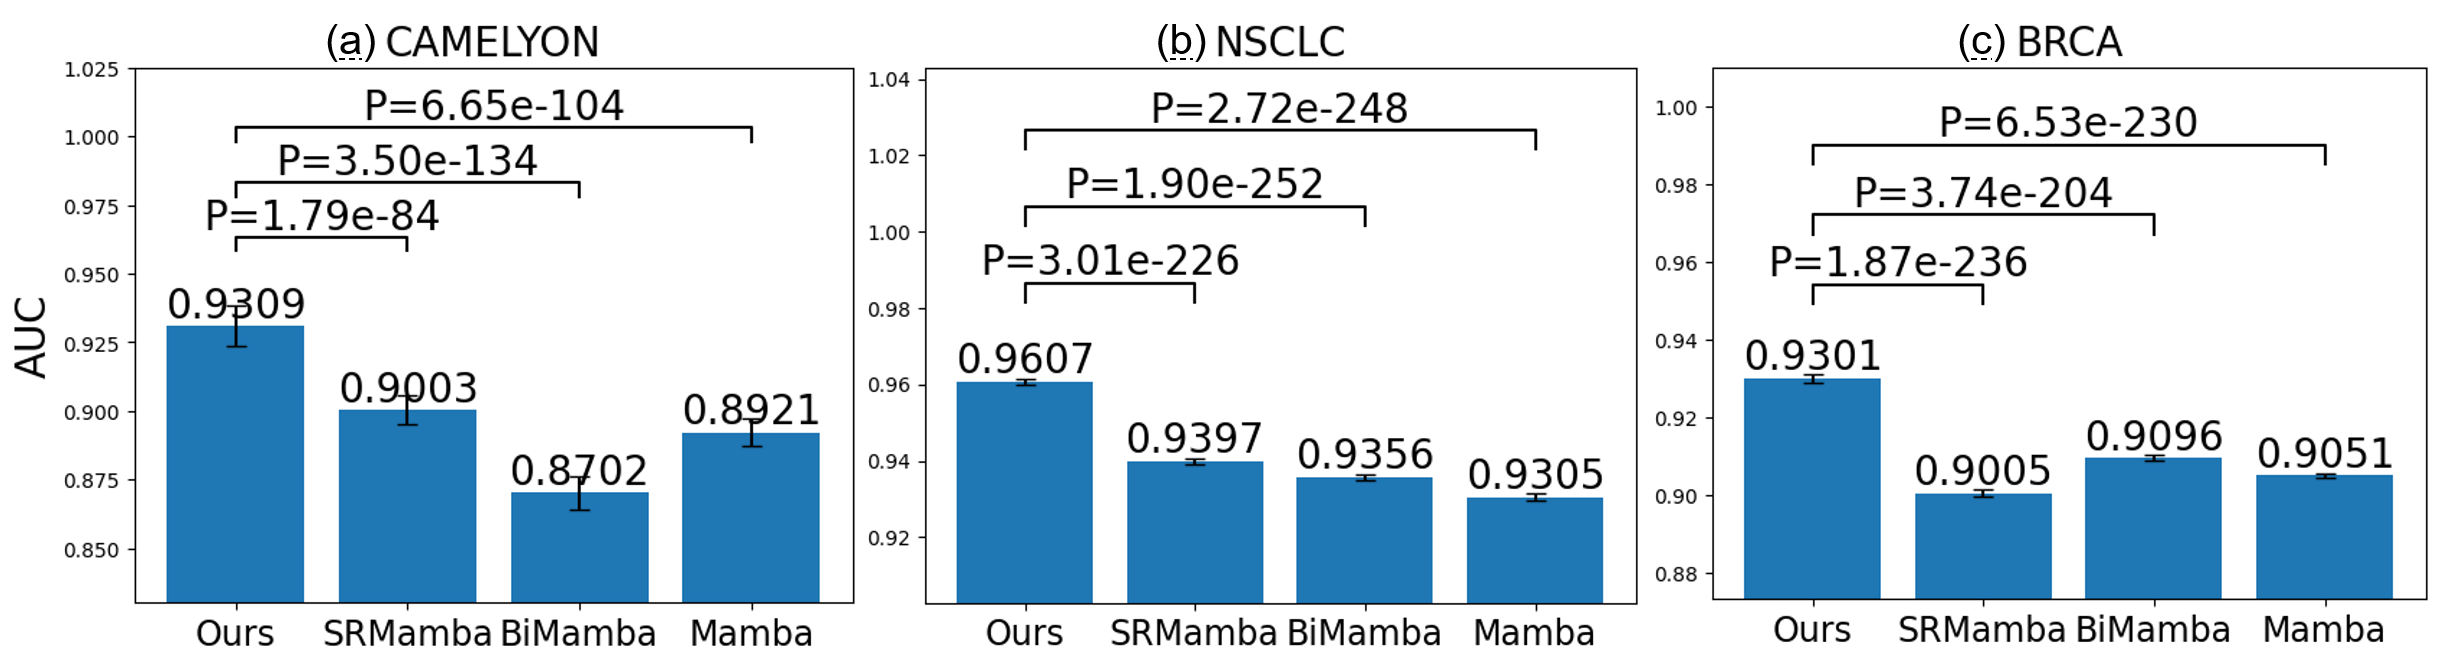
\includegraphics[width=1.0\columnwidth]{figures/scan_invariant.png}
  \bicaption[不同Mamba变体的扫描不变性评估的双样本t检验]{不同Mamba变体的扫描不变性评估的双样本t检验}[Two-sample t-test for scanning invariance evaluation of different Mamba variants]{Two-sample t-test for scanning invariance evaluation of different Mamba variants.}
  \label{figure4: scan-invariant}
  % \vspace{-4pt}
\end{figure}

为了验证本章的方法使Mamba能够构建更多的扫描不变性特征,本章将三个随机选择的扫描序列输入到训练的Mamba变体中进行推理,并分别计算其AUC的平均值和标准差。
实验结果见表\ref{table4: scan-invariant}。与基线相比,本章的方法在CAMELYON和NSCLC数据集上的标准差降低了2倍,在BRACS-7数据集上的标准差降低了3倍。
值得注意的是,本章的方法不仅在所有数据集中实现了最高的平均AUC,而且还显示出最小的标准差,并且与基准实验(表\ref{table4: CAMELYON}、\ref{table4: NSCLC}、\ref{table4: BRCA}和表\ref{table4: BRACS_7})中的正常输入的实验结果相差无几。
这强调了本章的方法在指导Mamba模型学习扫描序列的更多不变特征方面的有效性,优于其他Mamba变体方法。

为了进一步验证本章方法的扫描不变性,本章重复了验证过程,将随机化的数量增加到100,并进行了双样本t检验,如图\ref{figure4: scan-invariant}所示。结果显示,本章的方法不仅在平均值方面优于其他Mamba方法,而且p值远低于0.05。这表明,在统计意义上,其他Mamba方法与本章方法具有显著的差异。

\textbf{(3)不同Mamba模型性能比对}

\begin{figure}[h!]
  \centering
  \captionsetup{font={small, stretch=1.312}}
  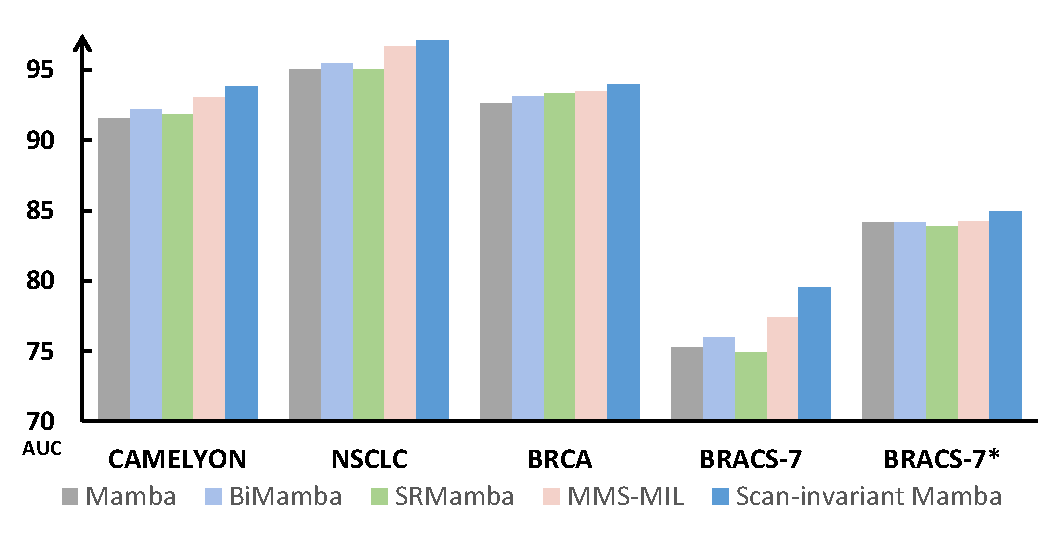
\includegraphics[width=0.9\columnwidth]{figures/SMCMIL的不同Mamba比较.pdf}
  \bicaption[不同Mamba模型性能比对柱状图]{不同Mamba模型性能比对柱状图。}[Bar chart of performance comparison of different Mamba models.]{Bar chart of performance comparison of different Mamba models.}
  \label{figure4: DifferentMamba}
  % \vspace{-4pt}
\end{figure}

为了进一步验证本章的方法的优越性来源于本章的架构而不是Mamba本身,本章对三种变体进行了比较实验:图\ref{figure4: DifferentMamba}中的Mamba Block、BiMamba和SRMamba。
结果表明,SMC-MIL在所有四个数据集上的所有六个任务中都取得了最佳性能。
本章的方法不仅在性能上超过了原始的单分支Mamba,而且在多序列(或扫描)聚合方法(例如,BiMamba和SRMamba,以及上一章提出的方法)中表现出许多优势。
实验结果表明,扫描不变Mamba算法比多扫描集成Mamba算法具有更强的实例建模能力,能够提取更多的判别性特征。


\textbf{(4)不同的分支对比策略对模型性能的影响}

\begin{table}[h!]
  \large    % 设置表格字体为5号
  \setstretch{1.245}        % 设置具有指定弹力的橡皮长度(原行宽的1.2倍)
  \captionsetup{font={small, stretch=1.512}}
  \centering
  % \vspace{-10pt}
  \bicaption[不同的分支对比策略对模型性能的影响]{不同的分支对比策略对模型性能的影响。最优结果使用粗体表示,次优结果使用下划线表示。}{Effects of different branch contrast strategies on model performance. The best results are shown in bold.}    % 中英文标题
  \begin{tabularx}{\textwidth}{lCCCC}
    \toprule
    方法 & CAMELYON& NSCLC& BRACS-3& BRACS-7\\ \midrule
  Vanilla vs. Hard & \underline{93.13$\pm$1.90} & 96.30$\pm$1.23 & 84.89$\pm$0.73 & \underline{76.52$\pm$0.32}\\
  Easy vs. Vanilla & 92.64$\pm$1.33 & \underline{96.55$\pm$1.21} & 82.66$\pm$4.39 & 77.44$\pm$0.95 \\
  Hard vs. Hard  &  90.39$\pm$2.55 & 95.79$\pm$1.48 & 82.57$\pm$1.83 & 77.22$\pm$2.65 \\
  Easy vs. Easy & 91.66$\pm$2.10 & 96.35$\pm$1.23  & \underline{85.63$\pm$0.84} & 74.48$\pm$1.61 \\ 
  \textbf{Easy vs. Hard} & \textbf{93.81$\pm$1.65} & \textbf{96.65$\pm$1.46} & \textbf{87.74$\pm$0.36} & \textbf{79.57$\pm$0.42} \\
    \bottomrule
  \end{tabularx}
  % \vspace{-25pt}
  \label{table4: Different branch}
\end{table}

表\ref{table4: Different branch}列出了五种不同分支对比策略下SMC-MIL的性能。结果表明,“Easy vs. Hard”策略产生最佳性能。
表现如此优异的主要原因是“Easy”分支帮助Mamba产生可靠的包表示和分类,而“hard”分支迫使模型不仅要学习扫描无关的特征,还要从被屏蔽序列中探索更多的判别实例,以实现两个分支之间的一致性。
此外,两个分支的差异也有利于性能提升。“Hard vs. Hard”策略表现最差。本章将其性能较差归因于在生成包表示和分类过程中缺乏来自“Easy”分支的可靠指导。

\textbf{(5)讨论不同扫描模式的组合对模型性能的影响}

\begin{table}[h!]
  \large    % 设置表格字体为5号
  \setstretch{1.245}        % 设置具有指定弹力的橡皮长度(原行宽的1.2倍)
  \captionsetup{font={small, stretch=1.512}}
  \centering
  % \vspace{-10pt}
  \bicaption[讨论不同扫描模式的组合对模型性能的影响]{讨论不同扫描模式的组合对模型性能的影响。最优结果用粗体表示。}{Effect of combinations of different scan patterns on model performance. The best results are shown in bold.}    % 中英文标题
  \begin{tabularx}{\textwidth}{lCCCC}
    \toprule
    方法 & CAMELYON& NSCLC& BRCA& BRACS-7$^\star$\\ \midrule
    Origin vs. Backward & {92.64$\pm$1.36} & \textbf{96.65$\pm$1.46} & \textbf{93.98$\pm$1.02} & \textbf{85.11$\pm$2.14} \\
    Origin vs. Random & \textbf{93.81$\pm$1.65} & {96.40$\pm$1.09} & {93.20$\pm$1.50} & {84.75$\pm$2.79} \\
    Origin vs. Grid. &  92.70$\pm$2.80 & 96.32$\pm$1.78 & 93.62$\pm$1.65 & 84.59$\pm$1.33 \\
    Origin vs. RSS. &  92.26$\pm$2.17 & 95.78$\pm$1.28 & 93.73$\pm$1.98 & 84.48$\pm$2.00 \\
    Random vs. Random  &  92.10$\pm$2.20 & 95.79$\pm$1.08 & 92.87$\pm$1.02 & 83.45$\pm$1.74 \\
    \bottomrule
  \end{tabularx}
  % \vspace{-25pt}
  \label{table4: Different scan}
\end{table}

比较不同的扫描模式可能会产生不同的结果。因此,本章还研究了使用不同形式的对比对SMC-MIL性能的影响。
如表\ref{table4: Different scan}所示,在CAMELYON数据集上,通过比较原始扫描模式和随机扫描模式可以获得最佳性能,而在其他数据集上,原始扫描模式和反向扫描模式可以获得最佳效果。
因此,在CAMELYON实验中,本章使用原始扫描模式和随机扫描模式来生成不同顺序的序列,对于剩余的数据集,本章使用原始扫描模式和反向扫描模式。
本小节同样对比了上一章提出的网格扫描和区域螺旋扫描模式,同样取得不错的性能。这侧面说明第三章提出的扫描模式补足了原始序列没有的空间信息。

\textbf{(6)讨论序列增强率的影响\texorpdfstring{$\alpha\%$}{}}

\begin{figure}[h!]
  \centering
  \captionsetup{font={small, stretch=1.312}}
  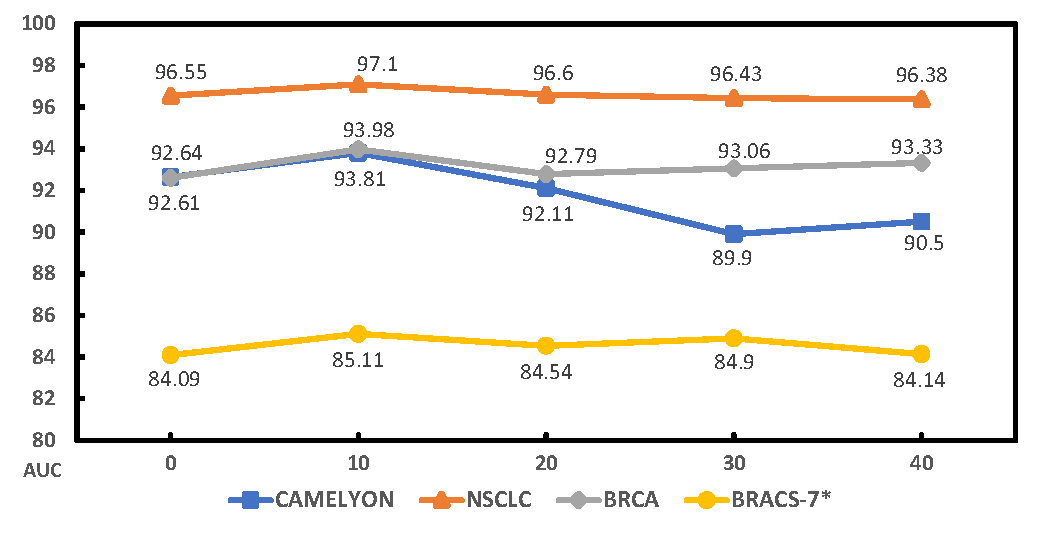
\includegraphics[width=0.8\columnwidth]{figures/MixRatio.pdf}
  \bicaption[不同序列增强率\texorpdfstring{$\alpha\%$}{}下的模型性能折线图]{不同序列增强率\texorpdfstring{$\alpha\%$}{}下的模型性能折线图。}[Line plot of model performance for different sequence enhancement rates \texorpdfstring{$\alpha\%$}{}]{Line plot of model performance for different sequence enhancement rates \texorpdfstring{$\alpha\%$}{}.}
  \label{figure4: mixratio}
\end{figure}

图\ref{figure4: mixratio}讨论了超参数序列增强率$\alpha\%$的影响。为了更好地突出实验结果,本章将BRACS-7$^\star$结果绘制在副轴上。
如图所示,除CAMELYON外,大多数数据集在序列增强率为0.1时达到最佳性能,CAMELYON在$\alpha\%=40\%$时达到峰值。为了保持一致性,本章将所有数据集的序列扩增率$\alpha\%$默认设置为$10\%$。


\textbf{(7)讨论序列掩码率的影响\texorpdfstring{$\beta\%$}{}}

\begin{figure}[h!]
  \centering
  \captionsetup{font={small, stretch=1.312}}
  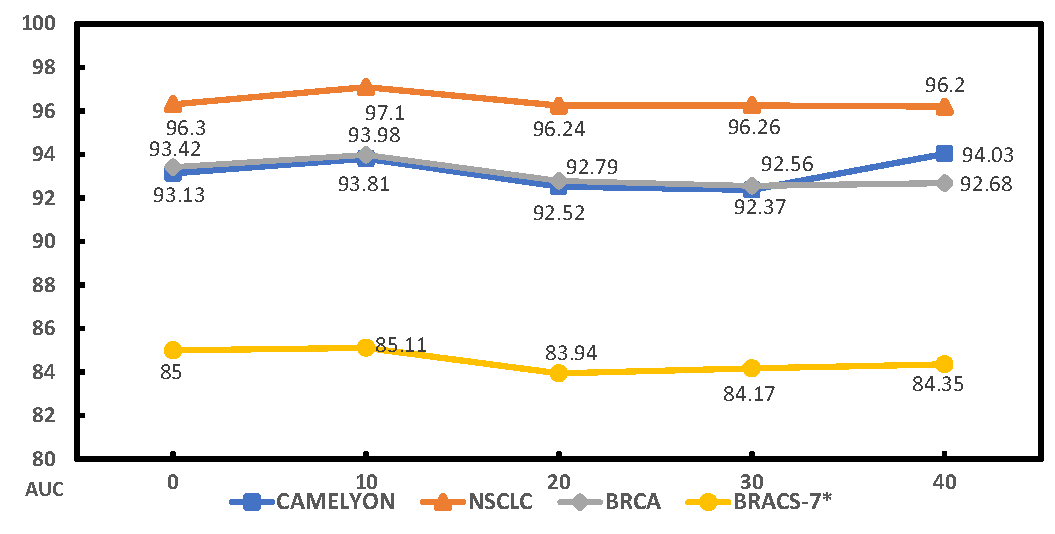
\includegraphics[width=0.8\columnwidth]{figures/MaskRatio.pdf}
  \bicaption[不同序列掩码率\texorpdfstring{$\beta\%$}{}下的模型性能折线图]{不同序列掩码率\texorpdfstring{$\beta\%$}{}下的模型性能折线图。}[Line plot of model performance for different sequence masking ratess \texorpdfstring{$\beta\%$}{}]{Line plot of model performance for different sequence masking ratess \texorpdfstring{$\beta\%$}{}.}
  \label{figure4: maskratio}
\end{figure}

图\ref{figure4: maskratio}讨论了超参数序列掩码率$\beta\%$的影响。本小节与前一小节一致,同样在次级轴上绘制了BRACS-7$^\star$结果。
所有数据集在$10\%$的序列掩码率下达到最佳性能。因此,除非另有说明,否则本章默认设置$\beta\% = 10\%$。

\textbf{(8)Bootstrap检验}

\begin{figure}[h!]
  \centering
  \captionsetup{font={small, stretch=1.312}}
  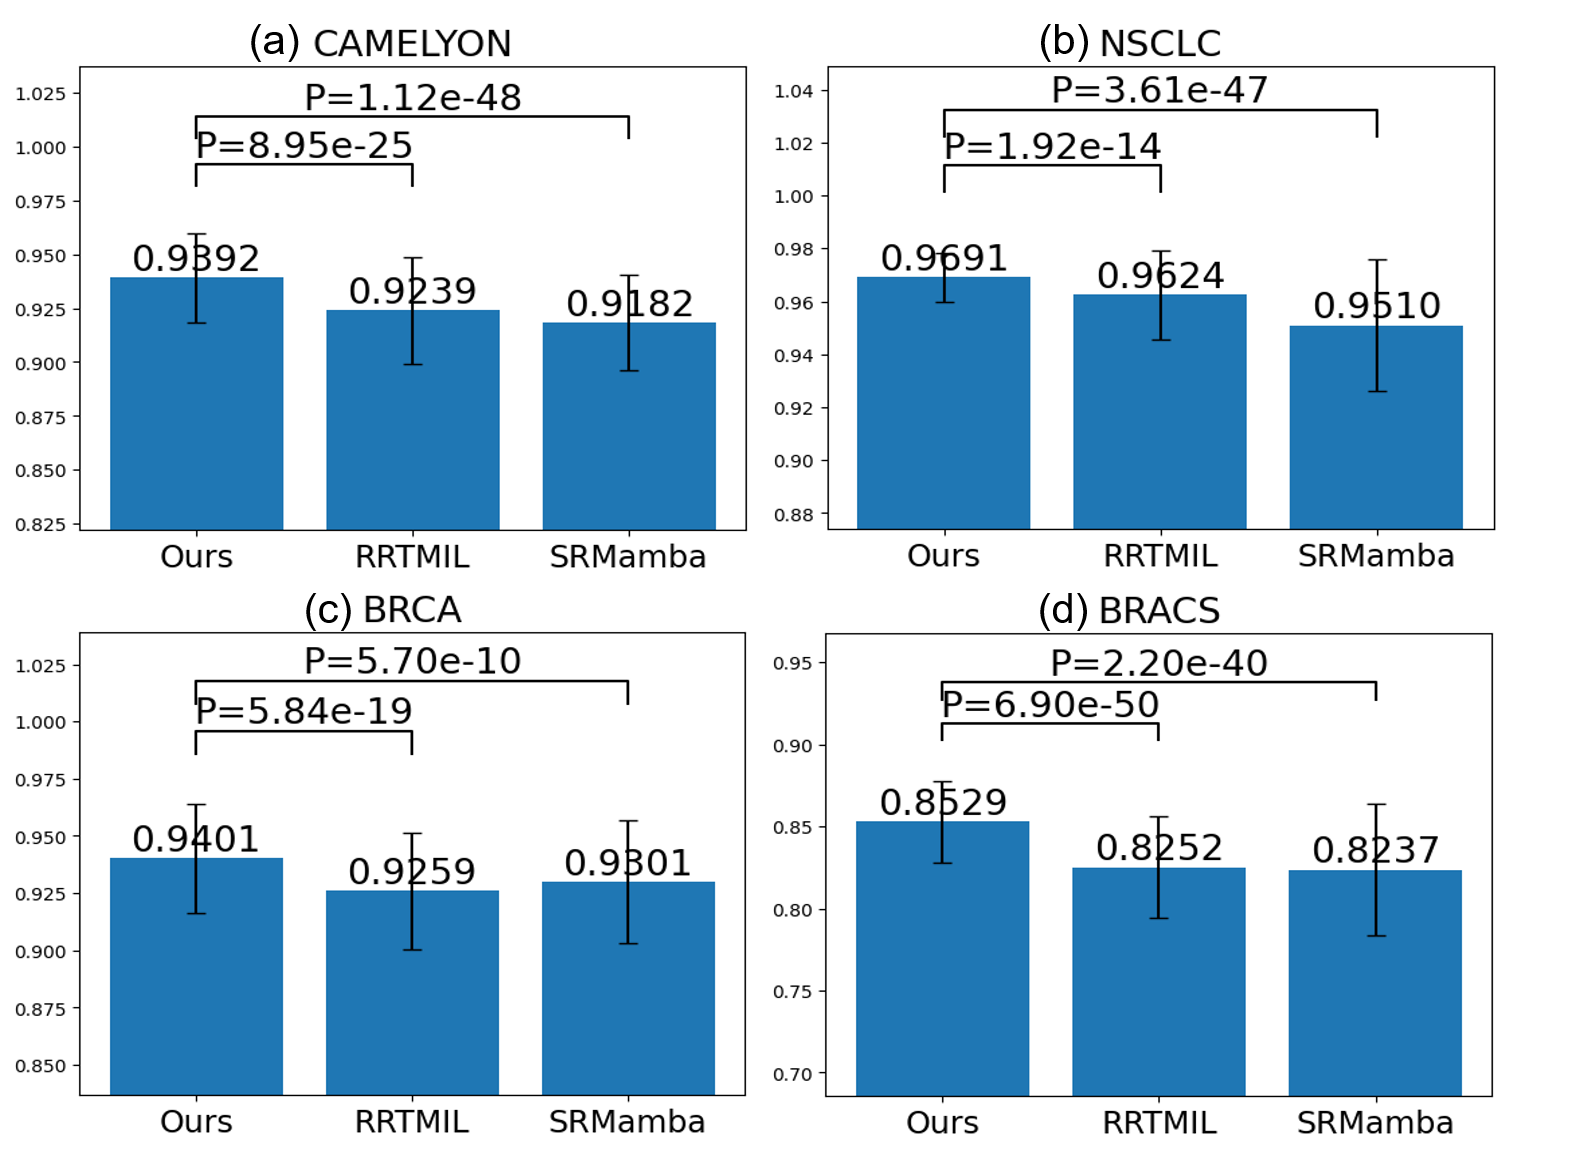
\includegraphics[width=0.8\columnwidth]{figures/t-testwithSOTA.png}
  \bicaption[与SOTA方法性能比较的Bootstrap检验]{与SOTA方法性能比较的Bootstrap检验。}[Bootstrap test for performance comparison with SOTA method]{Bootstrap test for performance comparison with SOTA method.}
  \label{figure4: sota t-test}
\end{figure}
本小节对本章方法和SOTA方法进行了有放回的随机抽样Bootstrap检验,共采样100次,得到的结果如图\ref{figure4: sota t-test}所示。可以看出,本章的方法显著高于SOTA,因为p值远小于0.05。

\textbf{(9)两种推理方式的性能对比}

\begin{table}[h!]
  \large    % 设置表格字体为5号
  \setstretch{1.245}        % 设置具有指定弹力的橡皮长度(原行宽的1.2倍)
  \captionsetup{font={small, stretch=1.512}}
  \centering
  % \vspace{-10pt}
  \bicaption[不同推理方式的性能对比]{不同的推理方式的性能对比。最优结果用粗体表示。}{Performance comparison of different inference modes. The best results are shown in bold.}    % 中英文标题
  \begin{tabularx}{\textwidth}{lCCCC}
    \toprule
    方法 & CAMELYON& NSCLC& BRACS-3& BRACS-7\\ \midrule
    w/ 序列增强模块 & \textbf{93.81$\pm$1.65} & 96.65$\pm$1.46 & \textbf{87.74$\pm$0.36} & \textbf{79.57$\pm$0.42} \\
    w/o 序列增强模块  & 93.70$\pm$1.42 & \textbf{96.67$\pm$1.31} & 87.65$\pm$4.17 & 79.43$\pm$0.95 \\
    \bottomrule
  \end{tabularx}
  % \vspace{-25pt}
  \label{table4: Different inference}
\end{table}
本小节讨论了使用不同推理方式对性能结果的影响,结果报告在表\ref{table4: Different inference}中。
可以看出两者并没有明显的差异,这更证明本章所提出模型的泛化性能。
默认设置下,本文采用有序列增强模块的推理模式进行推理。

\begin{table}[h!]
  \large    % 设置表格字体为5号
  \setstretch{1.245}        % 设置具有指定弹力的橡皮长度(原行宽的1.2倍)
  \captionsetup{font={small, stretch=1.512}}
  \centering
  % \vspace{-10pt}
  \bicaption[SMC-MIL以PLIP为离线特征提取器的癌症诊断性能]{SMC-MIL以PLIP为离线特征提取器的癌症诊断性能。最优结果用粗体表示,次优结果用下划线表示。}{Cancer diagnosis performance of SMC-MIL with PLIP as the offline feature extractors. The optimal experimental results are marked in bold, and the sub-optimal are underlined.}    % 中英文标题
  \begin{tabularx}{\textwidth}{clCCC}
    \toprule
    &方法  & Accuracy& AUC&F1-score\\ \midrule
    \multirow{6}{*}{\rotatebox{90}{PLIP}}&AB-MIL  & 90.09$\pm$1.63 & {94.55$\pm$1.91} & 86.48$\pm$2.50\\
    &OriginMamba        & 90.87$\pm$1.52 & 94.44$\pm$2.19 & 87.78$\pm$1.89\\
    &BiMamba          & 90.54$\pm$1.89 & 94.20$\pm$1.99 & 86.82$\pm$2.77\\
    &SRMamba & {91.87$\pm$0.85} & 94.20$\pm$2.16 & {88.37$\pm$1.31}\\
    &%\textbf{M$^2$S-MIL}
    第三章方法 & \underline{92.21$\pm$0.60} & \underline{95.24$\pm$1.85} & \underline{89.46$\pm$0.93}\\  
    &\textbf{SMC-MIL}        & \textbf{92.50$\pm$0.87} & \textbf{95.79$\pm$1.31} & \textbf{89.99$\pm$0.43}\\  
    \bottomrule
  \end{tabularx}
 \vspace{-25pt}
  \label{table4: CAMELYON_PLIP}
\end{table}
\begin{table}[h!]
  \large    % 设置表格字体为5号
  \setstretch{1.245}        % 设置具有指定弹力的橡皮长度(原行宽的1.2倍)
  \captionsetup{font={small, stretch=1.512}}
  \centering
  % \vspace{-10pt}
  \bicaption[SMC-MIL以PLIP为离线特征提取器在TCGA-NSCLC上的亚型分型性能]{SMC-MIL以PLIP为离线特征提取器在TCGA-NSCLC上的的亚型分型性能。最优结果用粗体表示,次优结果用下划线表示。}{Cancer sub-typing performance of SMC-MIL on the TCGA-NSCLC dataset with PLIP as the feature extractors. The optimal experimental results are marked in bold, and the sub-optimal experimental results are underlined.}    % 中英文标题
  \begin{tabularx}{\textwidth}{clCCC}
    \toprule
    &方法  & Accuracy& AUC&F1-score\\ \midrule
    \multirow{6}{*}{\rotatebox{90}{PLIP}}&AB-MIL  & 89.94$\pm$1.84 & 94.45$\pm$1.64 & 89.43$\pm$1.97\\
    &OriginMamba        & 90.89$\pm$1.60 & 95.57$\pm$1.60 & 90.24$\pm$1.84\\
    &BiMamba          & 90.70$\pm$1.95 & 95.42$\pm$1.68 & 89.94$\pm$2.26\\
    &SRMamba &  89.85$\pm$2.07 & 95.72$\pm$1.51 & 88.96$\pm$2.66 \\
    &%\textbf{M$^2$S-MIL}
    第三章方法  & \underline{91.56$\pm$1.76} & \underline{96.22$\pm$1.12} & \underline{90.64$\pm$1.86}\\     
    &\textbf{SMC-MIL}        & \textbf{92.30$\pm$0.60} & \textbf{96.78$\pm$1.68} & \textbf{91.79$\pm$0.50}\\  

    \bottomrule
\end{tabularx}
%\vspace{-25pt}

  \label{table4: NSCLC_PLIP}
\end{table}

\begin{table}[h!]
  \large    % 设置表格字体为5号
  \setstretch{1.245}        % 设置具有指定弹力的橡皮长度(原行宽的1.2倍)
  \captionsetup{font={small, stretch=1.512}}
  \centering
  % \vspace{-10pt}
  \bicaption[SMC-MIL以PLIP为离线特征提取器在TCGA-BRCA上的亚型分型性能]{SMC-MIL以PLIP为离线特征提取器在TCGA-BRCA上的亚型分型性能。最优结果用粗体表示,次优结果用下划线表示。}{Cancer sub-typing performance of SMC-MIL on the TCGA-BRCA dataset with PLIP as the feature extractors. The optimal experimental results are marked in bold, and the sub-optimal experimental results are underlined.}    % 中英文标题
  \begin{tabularx}{\textwidth}{clCCC}
    \toprule
    &方法  & Accuracy& AUC&F1-score\\ \midrule
    
    \multirow{6}{*}{\rotatebox{90}{PLIP}}&AB-MIL  & 83.81$\pm$3.72 & 90.18$\pm$2.99 & 67.94$\pm$4.22\\
  &OriginMamba        & 86.75$\pm$5.76 & 92.90$\pm$2.44 & 74.35$\pm$7.23\\
  &BiMamba          & 87.73$\pm$3.06 & 92.64$\pm$2.28 & 74.07$\pm$4.75\\
  &SRMamba & 86.40$\pm$3.31 & 92.17$\pm$2.67 & 72.39$\pm$4.62\\
  &%\textbf{M$^2$S-MIL} 
  第三章方法   & \underline{88.82$\pm$3.22} & \underline{93.40$\pm$1.24} & \underline{75.00$\pm$2.50}\\  
  &\textbf{SMC-MIL}        & \textbf{89.75$\pm$0.54} & \textbf{94.71$\pm$1.49} & \textbf{75.37$\pm$0.98}\\  

  \bottomrule
\end{tabularx}

  \label{table4: BRCA_PLIP}
\end{table}

\textbf{(10)使用PLIP作为特征提取器的性能结果}





\begin{figure}[h!]
  \centering
  \captionsetup{font={small, stretch=1.312}}
  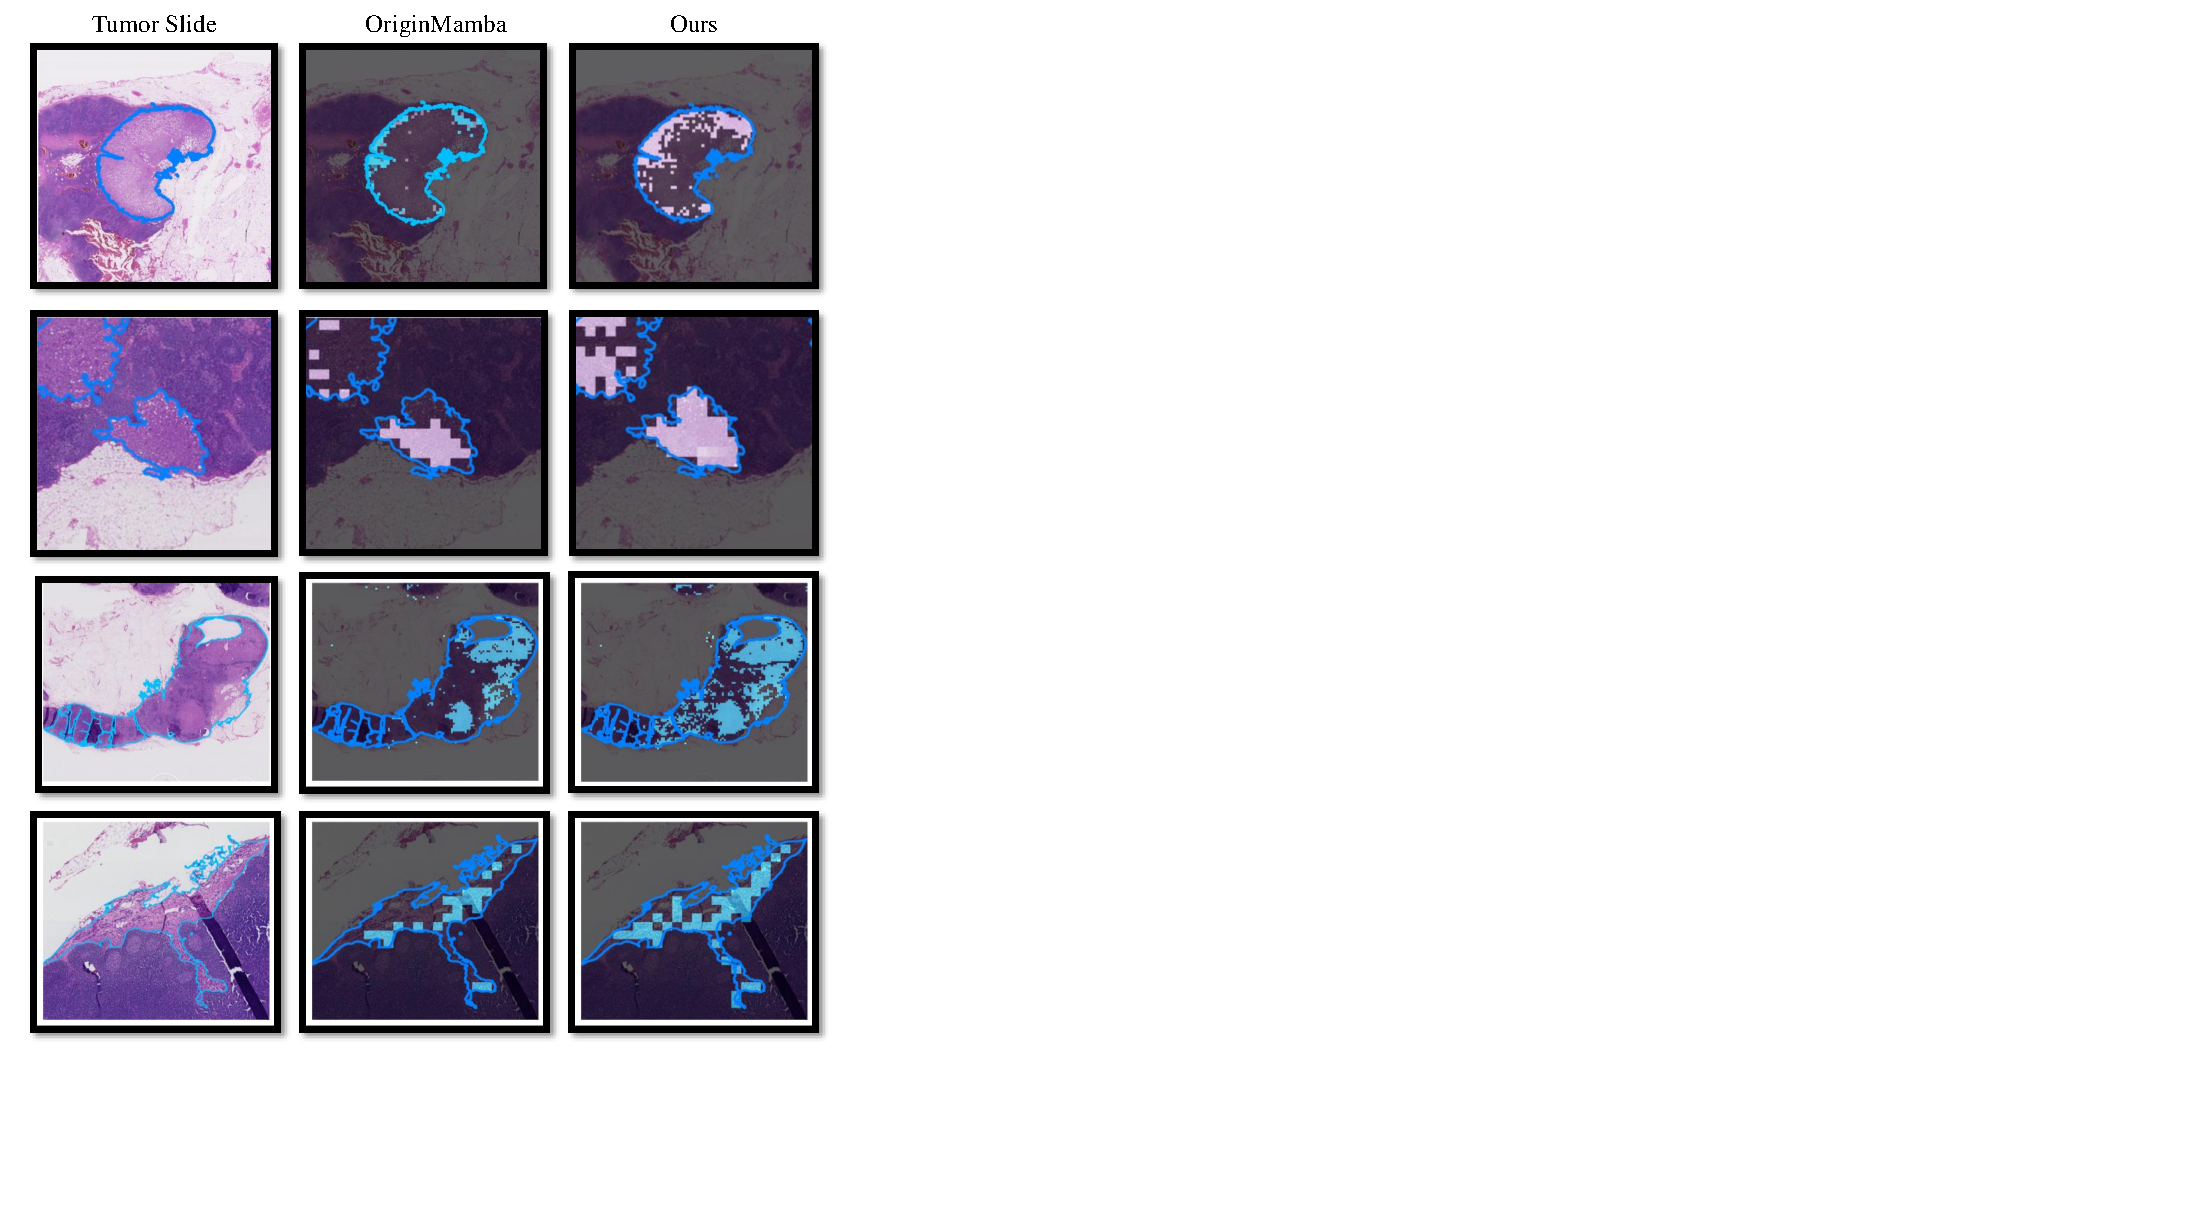
\includegraphics[width=0.8\columnwidth]{figures/Visualize_cropped.pdf}
  \bicaption[原始Mamba(baseline)和SMC-MIL关注的图块可视化结果]{原始Mamba(baseline)和SMC-MIL制作的图块可视化结果}[Visualization results of patches focused by original Mamba(baseline) and SMC-MIL]{Visualization results of patches focused by original Mamba(baseline) and SMC-MIL.}
  \label{figure4: visualize}
\end{figure}

\begin{figure}[h!]
  \centering
  \captionsetup{font={small, stretch=1.312}}
  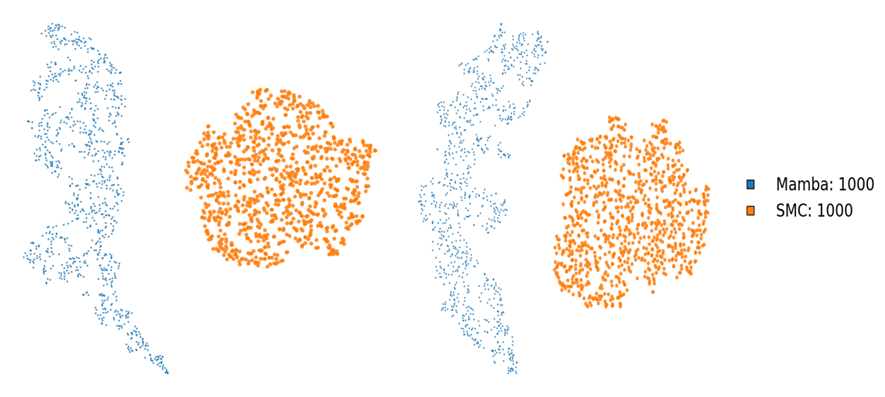
\includegraphics[width=0.8\columnwidth]{figures/t-SNE.png}
  \bicaption[原始Mamba(baseline)和SMC-MIL聚合特征t-SNE可视化结果]{原始Mamba(baseline)和SMC-MIL聚合特征t-SNE可视化结果}[The t-SNE visualization of aggregated features from original Mamba(baseline) and SMC-MIL]{The t-SNE visualization of aggregated features from Mamba(baseline) and SMC-MIL.}
  \label{figure4: tSNE}
\end{figure}


为了进一步探索本章方法的有效性,本小节还进行了将同样采用自监督预训练的PLIP~\cite{huang2023visual}作为特征提取器的相关实验,以验证本章方法的普遍适用性。
如表\ref{table4: CAMELYON_PLIP}、\ref{table4: NSCLC_PLIP}和\ref{table4: BRCA_PLIP}所示,可以看出实验结果与R50特征一致。
本章的方法优于其它基于Mamba的方法。在CAMELYON数据集上,它在精度、AUC和F1-score方面分别比次优的方法提高了0.29\%、0.55\%和0.53\%。这些指标在NSCLC数据集中分别为0.74\%,0.36\%和1.15\%。
最后,BRCA数据集的改进也值得注意,Acc提高了0.93\%,AUC提高了1.31\%,F1-score提高了0.37\%。
这进一步表明,即使使用非传统的ResNet-50特征提取器,本章方法的性能改进也不仅仅是依赖于简单的多个Mamba分支合并,而是正确捕获了空间信息与视觉特征。

\textbf{(11)Mamba效率优势的验证分析}

\begin{table}[h!]
  \large    % 设置表格字体为5号
  \setstretch{1.245}        % 设置具有指定弹力的橡皮长度(原行宽的1.2倍)
  \captionsetup{font={small, stretch=1.512}}
  \centering
  \vspace{-10pt}
  \bicaption[不同架构的性能与效率对比]{不同架构的性能与效率对比。}{Performance and efficiency comparison of different architectures.}    % 中英文标题
  \begin{tabularx}{\textwidth}{clCCC}
    \toprule
    &方法  & AUC(\%)& 训练时间(H) & 显存(G)\\ \midrule
    \multirow{6}{*}{\rotatebox{90}{CAMELYON}}&AB-MIL~\cite{ilse2018attention}  & 91.18$\pm$1.60 & \textbf{4.8} & \textbf{2.5}\\
    &Nystormer~\cite{xiong2021nystromformer}       & 91.23$\pm$1.82 & 10 & 15\\
    &ViT~\cite{dosovitskiy2020image} & - & - & OOM \\
    &Mamba~\cite{gu2023mamba}        & 91.57$\pm$1.37 & 5.5 & 6\\
    
    &SRMamba~\cite{yang2024mambamil}        & 91.82$\pm$0.93 & 6.8 & 7 \\
    &\textbf{SMC-MIL}        & \textbf{93.81$\pm$1.65} & 6 & 6.5 \\  
    \bottomrule
  \end{tabularx}
 \vspace{-10pt}
  \label{table4: efficiency}
\end{table}

为了充分验证Mamba架构相较于其他架构的优势,本章在相同设置下分别用单张GeForce RTX 3090测试了各架构在CAMELYON数据集上的实验所用训练时间、显存占用大小,并连同AUC报告在表\ref{table4: efficiency}。
其中Nystormer~\cite{xiong2021nystromformer}是一种经典的线性注意力变体,而OOM表示超出显存限制无法运行。由表\ref{table4: efficiency}可以看出,Mamba在病理图像分类领域不仅性能上有显著提升,而且在训练时间和显存占用上也具有很大优势。
这些结果也充分验证了本章所提出的方法在轻量化上的巨大优势。



\subsection[\hspace{-2pt}可视化分析]{{\heiti\zihao{4} \hspace{-8pt}可视化分析}}\label{section4: 可视化分析}






为了直观地验证本章方法的可解释性,本章将OriginMamba和本章的方法在Camelyon-16数据集上产生的高注意力分数的实例可视化,如图\ref{figure4: visualize}所示。蓝色的线条勾勒出肿瘤区域。越亮的斑块表明注意力得分越高。可视化结果清楚地表明,与原始Mamba相比,SMC-MIL能够更准确地选择显著斑块。
 
并且为了更加充分验证本章方法的扫描不变性,本章用t-SNE可视化了同一个WSI切片经过N个不同扫描模式所建模出的N个包特征,结果展示在图\ref{figure4: tSNE}(展示图中N为1000)。
可以看到SMC-MIL建模出的包特征明显更为集中,而原始Mamba的建模更为分散。实验充分说明本章所提出的基于序列差异化对比的Mamba模型具有扫描不变性。

\section[\hspace{-2pt}本章小结]{{\heiti\zihao{-3} \hspace{-8pt}本章小结}}\label{section4: 本章小结}

本章针对原始Mamba倾向性建模出因果关系与病理图像多实例学习的序列不变性存在冲突的问题,以引导Mamba建模与顺序无关的包特征为切入点,
提出了一种基于Mamba和对比学习的MIL框架,以解决扫描敏感Mamba和扫描不变MIL之间的差距。
该框架通过对不同扫描分支的结果应用一致性约束,指导Mamba从不同序列中学习包的扫描不变特征。
此外,序列对比度增强分别用于增强和掩码序列,迫使Mamba识别更多的鉴别斑块。
在3个WSI子任务以及12个基准上的大量对比及消融实验表明,该框架优于最新的其他方法,并且本章的方法解决了多扫描信息整合的策略存在无法穷举所有扫描情况,高度依赖扫描模式和集成方式的问题,有效地减轻了Mamba在MIL任务中的局限性,
使其更适合这些任务,并为Mamba在视觉任务中的进一步应用铺平了道路。
%未来,作者将致力于探索扫描不变性Mamba在更困难病理图像任务上的可能,如定位和分割。